\chapter[Notes on Data Structuring]{Notes on Data Structuring\footnote{This monograph is based on a series of lectures delivered at a Nato Summer School, Marktoberdorf, 1970.}}

{
	\noindent
	\scshape\hfill\scriptsize C. A. R. HOARE\hfill
}
\renewcommand{\leftmark}{\normalfont\scriptsize\hfill C. A. R. HOARE\hfill}

\section{Introduction}

In the development of our understanding of complex phenomena, the most powerful tool available to the human intellect is abstraction. Abstraction arises from a recognition of similarities between certain objects, situations, or processes in the real world, and the decision to concentrate on these similarities, and to ignore for the time being the differences. As soon as we have discovered which similarities are relevant to the prediction and control of future events, we will tend to regard the similarities as fundamental and the differences as trivial. We may then be said to have developed an abstract concept to cover the set of objects or situations in question. At this stage, we will usually introduce a word or picture to symbolize the abstract concept; and any particular spoken or written occurrence of the word or picture may be used to \textit{represent} a particular or general instance of the corresponding situation.

The primary use for representations is to convey information about important aspects of the real world to others, and to record this information in written form, partly as an aid to memory and partly to pass it on to future generations. However, in primitive societies the representations were sometimes believed to be useful in their own right, because it was supposed that manipulation of representations might in itself cause corresponding changes in the real world; and thus we hear of such practices as sticking pins into wax models of enemies in order to cause pain to the corresponding part of the real person. This type of activity is characteristic of magic and witchcraft. The modern scientist on the other hand, believes that the manipulation of representations could be used to predict events and the results of changes in the real world, although not to cause them. For example, by manipulation of symbolic representations of certain functions and equations, he can predict the speed at which a falling object will hit the ground, although he knows that this will not either cause it to fall, or soften the final impact when it does.

The last stage in the process of abstraction is very much more sophisticated; it is the attempt to summarize the most general facts about situations and objects covered under an abstraction by means of brief but powerful \textit{axioms}, and to prove rigorously (on condition that these axioms correctly describe the real world) that the results obtained by manipulation of representations can also successfully be applied to the real world. Thus the axioms of Euclidean geometry correspond sufficiently closely to the real and measurable world to justify the application of geometrical constructions and theorems to the practical business of land measurement and surveying the surface of the earth.

The process of abstraction may thus be summarized in four stages:

\begin{enumerate}[leftmargin=2\parindent, label=(\arabic*)]
	\item Abstraction: the decision to concentrate on properties which are shared  by many objects or situations in the real world, and to ignore the differences between them.
	\item Representation: the choice of a set of symbols to stand for the abstraction; this may be used as a means of communication.
	\item Manipulation: the rules for transformation of the symbolic representations as a means of predicting the effect of similar manipulation of the real world.
	\item Axiomatization: the rigorous statement of those properties which have been abstracted from the real world, and which are shared by manipulations of the real world and of the symbols which represent it.
\end{enumerate}

\subsection{Numbers and Numerals}
Let us illustrate this rather abstract description by means of a relatively concrete example --- the number four. In the real world, it is noticed that objects can be grouped together in collections, for example four apples. This already requires a certain act of abstraction, that is a decision to ignore (for the time being) the differences between the individual apples in the collection --- for example, one of them is bad, two of them unripe, and the fourth already partly eaten by birds.

Now one may consider several different collections, each of them with four items; for example, four oranges, four pears, four bananas, etc. If we choose to ignore the differences between these collections and concentrate on their similarity, then we can form a relatively abstract concept of the number four. The same process could lead to the concept of the number 3, 15, and so on; and a yet further stage of abstraction would lead to the development of the concept of a natural number.

Now we come to the representation of this concept, for example scratched on parchment, or carved in stone. The representation of a number is called a numeral. The early Roman numeral was clearly pictorial, just four strokes carved in stone: IIII. An alternative more convenient representation was IV. The arabic (decimal) representations are less pictorial, but again there is some choice: both 4 and 04 (and indeed 004 and so on) are all recognized as valid numerals, representing the same number.

We come next to a representation which is extremely convenient for processing, providing that the processor is an electronic digital computer. Here the number four is represented by the varying directions of magnetization of a group of ferrite cores. These magnetization are sometimes represented by sequences of zeros and ones on line printer paper; i.e., the binary representation of the number in question.

A simple example of the manipulation of numerals is addition, which can be used to predict the result of adjoining of two collections of objects in the real world. The addition rules for Roman numerals are very simple and obvious, and are simple to apply. The addition rules for arabic numerals up to ten are quite unobvious, and must be learnt; but for numbers much larger than ten they are more convenient than the Roman techniques. Addition of binary representations is not a task fit for human beings; but for a computer this is the simplest and best representation. Thus we see that choice between many representations can be made in the light of ease of manipulation in each particular environment.

Finally we reach the stage of axiomatization; the most widely known axiom set for natural numbers is that of Peano, which was first formulated at the end of the last century, long after natural numbers had been in general use. In the present day, the axiomatization of abstract mathematical ideas usually follows far more closely upon their development; and in fact may assist in the clarification of the concept by guarding against confusion and error, and by explaining the essential features of the concept to others. It is possible that a rigorous formulation of presuppositions and axioms on which a program is based may reduce the confusion and error so characteristic of present day programming practice, and assist in the documentation and explanation of programs and programming concepts to others.

\subsection{Abstraction and computer programming}

It is my belief that the process of abstraction, which underlies attempts to apply mathematics to the real world, is exactly the process which underlies the application of computers in the real world. The first requirement in designing a program is to concentrate on relevant features of the situation, and to ignore factors which are believed irrelevant. For example, in analyzing the flutter characteristics of a proposed wing design of an aircraft, its elasticity is what is considered relevant; its color, shape, and production technique are considered to be irrelevant except in so far as they have contributed to its elasticity. To take a commercial example, the employees working for a Company have many characteristics, both physical and mental, which will be ignored when devising a payroll program for the Company.

The next stage in program design is the decision of the manner in which the abstracted information is to be represented in the computer. An elasticity function may be represented by its values at a suitable number of discrete points; and these may be represented in a variety of ways as a two-dimensional array. Alternatively, the elasticity might be given by a computed function, and the data be held as a vector of polynomial or chebyshev coefficients for the function. A payroll file on a computer consists of a number of records, one relating to each employee. The choice of representation within the record of each relevant attribute must be made as part of the design of the program.

The stage of axiomatization is not usually regarded as a separate stage in programming; and is often left implicit. In the case of aircraft flutter, the axiomatization is the formulation of the differential equations which are presumed to describe the reaction of the real wing to certain kinds of stresses, and which (it is hoped) also describe the process of approximate solution on the computer. In the case of a payroll, the axioms correspond to the descriptions of various aspects of the real world which need to be embodied in the program --- for example, the fact that net pay equals gross pay minus deductions.

Finally there comes the task of programming the computer to get it to carry out those manipulations on the representation of the data that correspond to the manipulations in the real world in which we are interested. 

The success of a program is dependent on three basic conditions:

\begin{enumerate}[leftmargin=2\parindent, label=(\arabic*)]
	\item The axiomatisation is a correct description of those aspects of the real world with which it is concerned.
	\item The axiomatisation is a correct description of the behavior of the program, i.e., that the program contains no errors.
	\item The choice of representation and the method of manipulation are such that the cost of running the program on the computer is acceptable.
\end{enumerate}

In order to simplify the task of designing and developing a computer program, it is very helpful to be able to keep these three stages reasonably separate and to carry them out in the appropriate sequence. Thus the first stage (axiomatisation) would culminate in a rigorous logical statement of presuppositions about the real world, and a formulation of the desired objectives which are to be achieved by the program. The second stage would culminate in an algorithm, or abstract program, which is demonstrably capable of carrying out the stated task on the given presuppositions. The third stage would be the decision on how the various items of data are to be represented and manipulated in the store of the computer in order to achieve acceptable efficiency. Only when these three stages have been satisfactorily concluded will there begin the final phase of coding and testing the program, which embodies the chosen algorithm operating upon the chosen data representation.

Of course, this is a somewhat idealized picture of the intellectual task of programming as a steady progression from the abstract formulation of the problem to the more and more concrete aspects of its solution. In practice, even in the formulation of a problem, the programmer must have some intuition about the possibility of a solution; while he is designing his abstract program, he must have some feeling that an adequately efficient representation is available. Quite frequently these intuitions and feelings will be mistaken,
and a deeper investigation of representation, or even the final coding, will require a return to an earlier stage in the process, and perhaps even a radical recasting of the direction of attack. But this exercise of intuitive forethought, together with a risk of failure, is characteristic of all inventive and constructive intellectual processes, and does not detract from the merits of at least starting out in an orderly fashion, with more or less clearly separated stages.

One of the most important features of the progression is that the actual coding of the program has been postponed until after it is (almost) certain that all other aspects of the design have been successfully completed. Since coding and program testing is generally the most expensive stage in program development, it is undesirable to have to make changes after this stage has started. Thus it is advantageous to ensure beforehand that nothing further can go wrong at this final stage; for example, that the program tackles the right problem, that the algorithm is correct, that the various parts of the program cooperate harmoniously in the overall task, and that the data representations are adequately efficient. It is the purpose of this monograph to explore methods of achieving this confidence.

\subsection{Abstraction in high-level programming languages}

The role of abstraction in the design and development of computer programs may be reinforced by the use of a suitable high-level programming language. Indeed, the benefits of using a high-level language instead of machine code may be largely due to their incorporation of successful abstractions, particularly for data. To the hardware of a computer, and to a machine code programmer, every item of data is regarded as a mere collection of bits. However, to the programmer in ALGOL 60 or FORTRAN an item of data is regarded as an integer, a real number, a vector, or a matrix, which are the same abstractions that underlie the numerical application areas for which these languages were primarily designed. Of course, these abstract concepts have been mapped by the implementer of the language onto particular bit-pattern representations on a particular computer. But in the design of his algorithm, the programmer is freed from concern about such details, which for his purpose are largely irrelevant; and his task is thereby considerably simplified.

Another major advantage of the use of high-level programming languages, namely machine-independence, is also attributable to the success of their abstractions. Abstraction can be applied to express the important characteristics not only of differing real-life situations, but also of different computer representations of them. As a result, each implementer can select a representation which ensures maximum efficiency of manipulation on his particular computer.

A third major advantage of the use of a high-level language is that it significantly reduces the scope for programming error. In machine code programming it is all too easy to make stupid mistakes, such as using fixed point addition on floating point numbers, performing arithmetic operations on Boolean markers, or allowing modified addresses to go out of range. When using a high-level language, such errors may be prevented by three means:

\begin{enumerate}[leftmargin=2\parindent, label=(\arabic*)]
	\item Errors involving the use of the wrong arithmetic instructions are logically impossible; no program expressed, for example in ALGOL, could ever cause such erroneous code to be generated.
	\item Errors like performing arithmetic operations on Boolean markers will be immediately detected by a compiler, and can never cause trouble in an executable program.
	\item Errors like the use of a subscript out of range can be detected by runtime checks on the ranges of array subscripts.
\end{enumerate}

Runtime checks, although often necessary, are almost unavoidably more expensive and less convenient than checks of the previous two kinds; and high-level languages should be designed to extend the range of programming errors which logically cannot be made, or if made can be detected by a compiler. In fact, skillful language design can enable most subscripts to be checked without loss of runtime efficiency.

The automatic prevention and detection of programming errors may again be attributed to a successful appeal to abstraction. A high-level programming language permits the programmer to declare his intentions about the types of the values of the variables he uses, and thereby specify the meanings of the operations valid for values of that type. It is now relatively easy for a compiler to check the consistency of the program, and prevent errors from reaching the execution stage.

\subsection{Notations}

In presenting a theory of data structuring, it is necessary to introduce some convenient notation for expressing the abstractions involved. These notations are based to a large extent on those already familiar to mathematicians, logicians and programmers. They have also been designed for direct expression of computer algorithms, and to minimize the scope for programming error in running programs. Finally, the notations are designed to ensure the existence of efficient data representations on digital computers. Since the notations are intended to be used (among other things) for the expression of algorithms, it would be natural to conclude that they constitute a form of programming language, and that an automatic translator should be written for converting programs expressed in the language into the machine code of a computer, thereby eliminating the expensive and error-prone coding stage in the development of programs.

But this conclusion would be a complete misunderstanding of the reason for introducing the notations, and could have some very undesirable consequences. The worst of them is that it could lead to the rejection of the main benefits of the programming methodology expounded in this monograph, on the grounds that no compiler is available for the language, nor likely to be widely accepted if it were.

But there are sound reasons why these notations must not be regarded as a programming language. Some of the operations (e.g., concatenation of sequences), although very helpful in the design of abstract programs and the description of their properties, are grotesquely inefficient when applied to large data objects in a computer; and it is an essential part of the program design process to eliminate such operations in the transition between an abstract and a concrete program. This elimination will sometimes involve quite radical changes to both algorithm and representation, and could not in general be made by an automatic translator. If such expensive operators were part of a language intended for automatic compilation, it is probable that many programmers would fail to realize their obligation to eliminate them before approaching the computer; and even if they wanted to, they would have little feeling for what alternative representations and operations would be more economic. In taking such vital decisions, it is actually helpful if a programming language is rather close to the eventual machine, in the sense that the efficiency of the machine code is directly predictable from the form and length of the corresponding source language code.

There is a more subtle danger which would be involved in the automatic implementation of the notations: that the good programmer would soon learn that some of them are significantly less efficient than others, and he will avoid their use even in his abstract programs; and this will result in a form of mental block which might have serious consequences on his inventive capacity. Equally serious, the implementation of a fixed set of notations might well inhibit the user from introducing his own notations and concepts as required by his understanding of a particular problem.

Thus there is a most important distinction to be drawn between an algorithmic language intended to assist in the definition, design, development and documentation of a program, and the programming language in which the program is eventually conveyed to a computer. In this monograph we shall be concerned solely with the former kind of language. All example algorithms will be expressed in this language, and the actual coding of these programs is left as an exercise to the reader, who may choose for this purpose any language familiar to him, ALGOL, FORTRAN, COBOL, PL/I, assembly language, or any available combination of them. It is essential to a realization of the relative merits of various representations of data to realize what their implications on the resulting code will be.

In spite of this vigorous disclaimer that I am not embarking on the design of yet another programming language, I must admit the advantages that can follow if the programming language used for coding an algorithm is actually a \textit{subset} of the language in which it has been designed. I must also confess that there exists a large subset of the proposed algorithmic language which can be implemented with extremely high efficiency, both at compile time and at run time, on standard computers of the present day; and the challenge of designing computers which can efficiently implement even larger subsets may be taken up in the future. But the non-availability of such a subset implementation in no way invalidates the benefits of using the full set of notations as an abstract programming tool.

\subsection{Summary}

This introduction has given a general description of the motivation and general approach taken hereafter. As is quite usual, it may be read again with more profit on completion of the rest of the monograph.

The second section explains the concept of type, which is essential to the theory of data structuring; and relates it to the operations and representations which are relevant to the practice of computer programming.

Subsequent sections deal with particular methods of structuring data, progressing from the simpler to the more elaborate structures.

Each structure is explained informally with the aid of examples. Then the manipulation of the structure is defined by specifying the set of basic operations which may be validly applied to the structure. Finally, a range of possible computer representations is given, together with the criteria which should influence the selection of a suitable representation on each occasion.

Section 11 is devoted to an example, a program for constructing an examination timetable. The last section puts the whole exposition on a rigorous theoretical basis by formulating the axioms which express the basic properties of data structures. This section may be used as a summary of the theory, as a reference to refine the understanding, or as a basis for the proof of correctness of programs.

\section[The concept of type]{The Concept Of Type}

The theory of data structuring here propounded is strongly dependent on the concept of type. This concept is familiar to mathematicians, logicians, and programmers.

(1) In mathematical reasoning, it is customary to make a rather sharp distinction between individuals, sets of individuals, families of sets, and so on; to distinguish between real functions, complex functions, functionals, sets off unctions, etc. In fact for each new variable introduced in his reasoning, a mathematician usually states immediately what type of object the variable can stand for, e.g.

\quad ``Let $f$ be a real function of two real variables''

\quad ``Let $S$ be a family of sets of integers''.

Sometimes in mathematical texts a general rule is given which relates the type of a symbol with a particular printer's type font, for example:

\hangindent=1.9\parindent \quad``We use small Roman letters to stand for individuals, capitals to stand for sets of individuals, and script capitals to denote families of sets''.

In general, mathematicians do not use type conventions of this sort to make distinctions of an arbitrary kind; for example, they would not be generally used to distinguish prime numbers from non-primes or Abelian groups from general groups. In practice, the type conventions adopted by mathematicians are very similar to those which would be of interest to logicians and programmers.

(2) Logicians on the whole prefer to work without typed variables. However without types it is possible to formulate within set theory certain paradoxes which would lead to inescapable contradiction and collapse of logical and mathematical reasoning. The most famous of these is the Russell paradox:

\quad \hspace{-.4em}``let $s$ be the set of all sets which are \textit{not} members of themselves.

\quad Is $s$ a member of itself or not?''

\noindent
It turns out that whether you answer yes or no, you can be immediately proved wrong.

Russell's solution to the paradox is to associate with each logical or mathematical variable a \textit{type}, which defines whether it is an individual, a set, a set of sets, etc. Then he states that any proposition of the form ``$x$ is a member of $y$'' is grammatically meaningful only if $x$ is a variable of type individual and $y$ a variable of type set, or if $x$ is of type set and $y$ is of type set of sets, and so on. Any proposition that violates this rule is regarded as meaningless --- the question of its truth or falsity just does not arise, it is just a jumble of letters. Thus any proposition involving sets that are or are not members of themselves can simply be ruled out.

Russell's theory of types leads to certain complexities in the foundation of mathematics, which are not relevant to describe here. Its interesting features for our purposes are that types are used to prevent certain erroneous expressions from being used in logical and mathematical formulae; and that a check against violation of type constraints can be made merely by scanning the text, without any knowledge of the value which a particular symbol might happen to stand for.

(3) In a high-level programming language the concept of a type is of central importance. Again, each variable, constant and expression has a unique type associated with it. In ALGOL 60 the association of a type with a variable is made by its declaration; in FORTRAN it is deduced from the initial letter of the variable. In the implementation of the language, the type information determines the representation of the values of the variable, and the amount of computer storage which must be allocated to it. Type information also determines the manner in which arithmetic operators are to be interpreted; and enables a compiler to reject as meaningless those programs which invoke inappropriate operations.

Thus there is a high degree of commonality in the use of the concept of type by mathematicians, logicians and programmers. The salient characteristics of the concept of type may be summarized:

\begin{enumerate}[leftmargin=2\parindent, label=(\arabic*)]
	\item A type determines the class of values which may be assumed by a variable or expression.
	\item Every value belongs to one and only one type.
	\item The type of a value denoted by any constant, variable, or expression may be deduced from its form or context, without any knowledge of its value as computed at run time.
	\item Each operator expects operands of some fixed type, and delivers a result of some fixed type (usually the same). Where the same symbol is applied to several different types (e.g. $+$ for addition of integers as well as reals), this symbol may be regarded as ambiguous, denoting several different actual operators. The resolution of such systematic ambiguity can always be made 	at compile time.
	\item  The properties of the values of a type and of the primitive operations defined over them are specified by means of a set of axioms.
	\item Type information is used in a high-level language both to prevent or detect meaningless constructions in a program, and to determine the method of representing and manipulating data on a computer.
	\item The types in which we are interested are those already familiar to mathematicians; namely, Cartesian Products, Discriminated Unions, Sets, Functions, Sequences, and Recursive Structures.
\end{enumerate}

\subsection{Data type definitions}

Our theory of data structuring specifies a number of standard methods of defining types, and of using them in the declaration of variables to specify the range of values which that variable may take in the course of execution of a program. In most cases, a new type is defined in terms of previously defined \textit{constituent} types; the values of such a new type are data structures, which can be built up from \textit{component} values of the constituent types, and from which the component values can subsequently be extracted. These component values will belong to the constituent types in terms of which the structured type was defined. If there is only one constituent type, it is known as the \textit{base} type.

The number of different values of a data type is known as its \textit{cardinality}. In many cases the cardinality of a type is finite; and for a structured type defined in terms of finite constituent types, the cardinality is also usually finite, and can be computed by a simple formula. In other cases, the cardinality of a data type is infinite, as in the case of integers; but it can never be more than denumerably infinite. The reason for this is that each value of the type must be constructible by a finite number of computer operations, and must be representable in a finite amount of store. Arbitrary real numbers, functions with infinite domains. and other classes of non-denumerable cardinality can never be represented as stored data within a computer, though in some cases they can be represented by procedures, functions, or other program structures.

Obviously, the ultimate components of a structure must be unstructured, and the ultimate constituents of a structured type must be unstructured types. One method of defining an unstructured type is by simple enumeration of its values, as described in the next section. But in certain cases it is better to regard the properties of unstructured types as defined by axioms, and assume them to be provided as \textit{primitive} types by the hardware of a computer or the implementation of a high-level programming language. For example, the primitive types of ALGOL 60 are \textbf{integer}, \textbf{real}, and \textbf{Boolean}, and these will be assumed available.

\subsection{Data manipulation}

The most important practical aspect of data is the manner in which that data can be manipulated, and the range of basic operators available for this purpose. We therefore associate with each type a set of \textit{basic} operators which are intended to be useful in the design of programs, and yet which have at least one reasonably efficient implementation on a computer. Of course the selection of basic operators is to some extent arbitrary, and could have been either larger or smaller. The guiding principle has been to choose a set large enough to ensure that any additional operation required by the programmer can be defined in terms of the basic set, and be efficiently implemented in this way also; so an operator is regarded as basic if its method of efficient implementation depends heavily on the chosen method of data representation.

The most important and general operations defined for data of any type are assignment and test of equality. Assignment involves conceptually a complete copy of a data value from one place to another in the store of the computer; and test of equality involves a complete scan of two values (usually stored at different places) to test their identity. These rules are those that apply to primitive data types and there is no reason to depart from them in the case of structured types. If the value of a structured type is very large, these operations may take a considerable amount of time; this can sometimes be reduced by an appropriate choice of representation; alternatively, such operations can be avoided or removed in the process of transforming an abstract program to a concrete one.

Another general class of operators consists in the \textit{transfer} functions, which map values of one type into another. Of particular importance are the \textit{constructors}, which permit the value of a structured type to be defined in terms of the values of the constituent types from which it is built. The converse transfer functions are known as \textit{selectors}; they permit access to the component values of a structured type. In many cases, we use the name of a defined type as the name of the standard constructor or transfer function which ranges over the type.

Certain data types are conveniently regarded as ordered; and comparison operators are available to test the values of such types. But for many types, such an ordering would have no meaningful interpretation; and such types are best regarded from an abstract point of view as unordered. This will sometimes be of advantage in giving greater freedom in the choice of representation and sequencing strategies at a later state in the concrete design.

In the case of a large data structure, the standard method of operating efficiently on it is not by assigning a wholly new value to it, but rather by \textit{selectively updating} some relatively small part of it. The usual notation for this is to write on the left of an assignment an expression (variable) which uses selectors to denote the place where the structure is to be changed. However, we also introduce special assignment operators, always beginning with colon, to denote other more general updating operations such as adding a member to a set, or appending an item to a sequence. For both kinds of selective updating, it must be remembered that, from a conceptual or abstract point of view, the entire value of the variable has been changed by updating the least part of it.

\subsection{Representations}

It is fundamental to the design of a program to decide how far to store computed results as data for subsequent use, and how far to compute them as required. It is equally fundamental to decide how stored data should be represented in the computer. In many simple and relatively small cases there is an obvious \textit{standard} way of representing data, which ensures that not too much storage is used, and not too much time expended on carrying out the basic operations. But if the volume of data (or the amount of processing) is large, it is often profitable (and sometimes necessary) to choose some non-standard representation, selected in accordance with the characteristics of the storage media used (drums, discs, or tapes), and also taking into account the relative frequencies of the various operations which will be performed upon it. Decisions on the details of representation must usually precede and influence the design of the code to manipulate the data, often at a time when the nature of the data and the processing required are relatively unknown. Thus it is quite common to make serious errors of judgment in the design of data representation, which do not come to light until shortly before, or even after, the program has been put into operation. By this time the error is extremely difficult to rectify. However, the use of abstraction in data structuring may help to postpone some of the decisions on data representation until more is known about the behavior of the program and the characteristics of the data, and thus make such errors less frequent and easier to rectify.

An important decision to be taken is on the degree and manner in which data should be compressed in storage to save space; and also to save time on input$/$output, on copying operations, and on comparisons, usually at the expense of increasing the time and amount of code required to perform all other operations. Representations requiring less storage than the standard are usually known as \textit{packed}; there are several degrees of packing, from loose to tight. Of theoretical interest is the \textit{minimal} representation, which uses the least possible space. In this representation the values of the type are represented as binary integers in the range 0 to $N - 1$, where $N$ is the cardinality of the type. In the case of a type of infinite cardinality, a minimal representation is one in which every possible bit pattern represents a value of the type. Minimal representations are not often used, owing to the great expense of processing them.

Another method of saving space is to use an \textit{indirect} representation. In the standard direct representation of data, each variable of a type is allocated enough space to hold every value of the type. In the indirect representation, the variable is just large enough to contain a single machine address, which at any given time points to a group of one or more machine locations containing the current value. This technique is necessary when the type has infinite cardinality, since the amount of storage used will vary, and is not known when writing the code which accesses the variable. It can also be profitable when the actual amount of storage is variable, and during a large part of a program run is significantly less than the maximum. Finally, it can be used when it is believed that many different variables will tend to have the same values; since then only one copy of the value need be held, and the variables may just contain pointers to it; copying the value is also very cheap, since only the pointer need be copied. However, such shared copies must never be selectively updated.

Unfortunately, indirect representations often involve the additional expense and complexity of a dynamic storage allocation and garbage collection scheme; and they can cause some serious problems if data has to be copied between main and backing stores.

This chapter describes only a small but useful range of the possible representations of data, and the skillful programmer could readily add to the selection. In many cases, the representation of an abstract data type can be constructed by means of a more elaborate but more efficient data type definition; for instance a large set may be represented as a sequence of items of some suitable type. Examples of this are given in later sections.

\section[Unstructured data types]{Unstructured Data Types}
\label{sec:unstructured-data-types}

All structured data must in the last analysis be built up from unstructured components, belonging to a primitive or unstructured type. Some of these unstructured types (for example, reals and integers) may be taken as given by a programming language or the hardware of the computer. Although these primitive types are theoretically adequate for all purposes, there are strong practical reasons for encouraging a programmer to define his own unstructured types, both to clarify his intentions about the potential range of values of a variable, and the interpretation of each such value; and to permit subsequent design of an efficient representation.

In particular, in many computer programs an integer is used to stand not for a numeric quantity, but for a particular choice from a relatively small number of alternatives. In such cases, the annotation of the program usually lists all the possible alternative values, and gives the intended interpretation of each of them. It is possible to regard such a quantity as belonging to a separate type, quite distinct from the integer type, and quite distinct from any other similar set of markers which have a different interpretation. Such a type is said to be an \textit{enumeration}, and we suggest a standard notation for declaring the name of the type and associating a name with each of its alternative values:
\medskip

\tabto{3.7em}\textbf{type} suit $=$ (club, diamond, heart, spade);

\noindent
\hangindent=5.6\parindent\textbf{ordered} \tabto{3.7em}\textbf{type} rank = (two, three, four, five, six, seven, eight, nine, ten, Jack, Queen, King, Ace);
\medskip

\tabto{3.7em}\textbf{type} primary color $=$ (red, yellow, blue);

\noindent
\hangindent=7.4\parindent\textbf{ordered} \tabto{3.7em}\textbf{type} day of week $=$ (Monday, Tuesday, Wednesday, Thursday, Friday, Saturday, Sunday);
\medskip

\tabto{3.7em}\textbf{type} day of month $= 1\,.\,.\,31$;

\noindent
\hangindent=6.2\parindent\textbf{ordered} \tabto{3.7em}\textbf{type} month $=$ (Jan, Feb, March, April, May, June, July, Aug, Sept, Oct, Nov, Dec);
\medskip

\tabto{3.7em}\textbf{type} year $= 1900\,.\,.\,1969$;

\tabto{3.7em}\textbf{type} Boolean $=$ (false, true);
\medskip

\noindent
\hangindent=5.6\parindent\textbf{ordered} \tabto{3.7em}\textbf{type} floor $=$ (basement, ground, mezzanine, first, second);

\tabto{3.7em}\textbf{type} coordinate $= 0\,.\,.\,1023$;
\medskip

Our first two examples are drawn from the realm of playing cards. The first declaration states that club, diamond, heart, and spade are suits; in other words, that any variable or expression of type suit can only denote one of these four values; and that the identifiers ``club'' ``heart'' ``diamond'' and ``spade'' act as \textit{constants} of this type. Similarly, the definition of the type \textit{rank} displays the thirteen constants denoting the thirteen possible values of the type. In this case it is natural to regard the type as ordered. The next examples declare the names of the primary colors and of the days of the week. In considering the days of the month, it is inconvenient to write out the thirty-one possible values in full. We therefore introduce the convention that $a\,.\,.\,b$ stands for the finite range of values between $a$ and $b$ inclusive. This is known as a \textit{subrange} of the type to which $a$ and $b$ belong, in this case integers. This convention is used again in the declaration of year. Other examples of enumeration are:

\quad The Boolean type, with only two values, false and true.

\quad The Month type, with twelve values listed in the required order.

\hangindent=2.8\parindent\quad The coordinate type, taking values between 0 and 1023, representing perhaps a coordinate on a CRT display.

Having defined a type in a suitable fashion, the programmer will use the type name to specify the types of his variables. For this purpose it is useful to follow the current practice of mathematicians and to write the type name \textit{after} the variable, separated from it by a colon:

\quad trumps: suit; today:day of week;

\quad $pc$: primary color;

\noindent
If several variables of the same type are to be declared at the same time, it is useful to adopt the abbreviation of listing the variable names without repeating the type name, thus:

\quad arrival, departure: day of month;

\quad $x$, $y$, $z$: coordinate.

\noindent
If only a few variables of a given type are to be used, it is convenient to write the type definition itself in place of and instead of the type name:

\quad answer: (yes, no, don't know);

The cardinality of a type defined by enumeration is obviously equal to the length of the defining list; and for a numeric subrange, it is one more than the difference between the end points of the subrange.

\subsection{Manipulation}

The operations required for successful manipulation of values of enumeration types and subranges are:

\begin{enumerate}[leftmargin=2\parindent, label=(\arabic*)]
	\item test of equality, for example:

	\quad \textbf{if} arrival $=$ departure \textbf{then go} to transit desk;

	\quad \textbf{if} trumps $=$ spade \textbf{then} \dots

	\item assignment, for example·

	\quad $pc \coloneq$ yellow;

	\quad trumps $\coloneq$ club;

	\item \label{en:manipulation-3}
	case discrimination, for example:

	\quad \textbf{case} $p$c \textbf{of} (red: \dots,

	\tabto{5.7em}yellow: \dots,

	\tabto{5.7em}blue: \dots)
	
	where $pc$ is a variable or expression of type primary color, and the limbs of the discrimination are indicated by lacunae. A case discrimination may be either a statement, in which case the limbs must be statements; or it may be an expression, in which case the limbs must be all expressions of the same type.
	
	The effect of a case discrimination is to select for execution (or evaluation) that single statement (or expression) which is prefixed by the constant equal to the current value of the case expression. In some cases, it may be convenient to prefix several constants to the same limb, or even to indicate a subrange of values which would select the corresponding limb; but of course each value must be mentioned exactly once:
	
	\quad \textbf{case} digit \textbf{of} ($0\,.\,.\,2:\dots$,
	
	\tabto{6.6em}$3:7:\dots$,
	
	\tabto{6.6em}$4\,.\,.\,6:8:9:\dots$).
	
	\noindent
	In this last case, it would be convenient to replace the labels of the last limb by the basic word \textbf{else}, to cover all the remaining cases not mentioned explicitly on the preceding limbs.
	
	When the limbs of a discrimination are statements, we shall sometimes use braces instead of brackets to surround them.
	
	\item In the case of a type declared as ordered, it is possible to test the ordering relationships among the values:
	
	\quad \textbf{if} May $\leqslant$ this month \& this month $\leqslant$ September \textbf{then}
	
	\qquad adopt summer timetables. 
	
	\noindent
	In other cases, the ordering of the values is quite irrelevant, and has no meaning to the programmer.
	
	\item In conjunction with ordering, it is useful to introduce a successor and a predecessor function (succ and pred) to map each value of the type onto the next higher or lower value, if there is one. Also, if $T$ is any ordered type, the notation $T$.min will denote the lowest value of the type, and $T$.max the highest value, if they exist. This helps in formulating programs, theorems, and axioms in a manner independent of the actual names of the constants.
	\item In a computer program we will frequently wish to cause a variable to range sequentially all through the values of a type. This may be denoted by a
	
	form of for statement or loop
	
	\textbf{for} $a:\text{alpha}$ \textbf{do} \dots;
	
	\textbf{for} $i:1\,.\,.\,99$ \textbf{do} \dots;
	
	In this construction, the counting variable ($a$ or $i$) is taken to belong to the type indicated, and to be declared locally to the construction, in the sense that its value does not exist before or after the loop, and its name is not accessible outside the loop. In addition, the value of the counting variable is not allowed to be changed inside the body of the loop, since this would frustrate the whole intention of declaring the variable by means of the \textbf{for} construction.
	
	In the case of an ordered type, it is natural to assume that the counting variable sequences through the values of the type in the defined order, $T.$min, succ($T.$min), \dots, $T.$max. But if the type is an unordered one, it is assumed that the sequence of the scan does not matter at the current level of abstraction, and will be defined at some later stage in the development of a concrete program.
	
	\item For subrange types, particularly integer subranges, it is sometimes required to perform operations which are defined for the original larger type. In principle, it is simple to accomplish this by first converting the subrange value to the corresponding value of the larger type, and then performing the operation, and finally converting back again if necessary. This requires a type transfer function; and for this purpose it is convenient to use the name of the destination type, for example:
	
	\quad $x$distance $\coloneq$ integer($x$) - integer($y$);
	
	\quad z $\coloneq$ coordinate(integer($z$) $+$ $x$distance);
	
	where $x$distance is an integer variable. Of course, this is an excessively cumbersome notation, and one would certainly wish to adopt the convention of omitting the conversions, where the need for their re-insertion can be established from the context:
	
	$x$distance $\coloneq x - y$;
	
	$z \coloneq z + x$distance.
\end{enumerate}

\noindent
\textit{Exercise}

\noindent
Given $m$:month and $y$:year, write a case discrimination expression giving the number of days in month $m$.

\subsection{Representation}

The standard representation of an enumeration type $T$ is to map the values in the stated order onto the computer integers in the range 0 to $n - 1$, where $n$ is the cardinality of the type. Thus in this case the standard representation is also minimal. The standard representation of a subrange is to give each value the same representation that it had in the original type; thus transfer between the types involves no actual operation; though of course conversion from the base type to the subrange type should involve a check to ensure that the value is within the specified range.

The minimal representation of a subrange value is obtained by subtracting from the standard form the integer representation of the least value of the subrange. In this case, conversion to a subrange involves subtraction as well as a check, and conversion in the opposite direction involves an addition.

Apart from these conversions, enumerations and subranges in either representation can be treated identically. Tests of ordering can be accomplished by normal integer instructions of the computer, and succ and pred involve addition or subtraction of unity, followed by a test that the result is still within range.

The case discrimination can be most efficiently carried out by a switch-jump. For example, in ALGOL 60 the first example quoted above (3.1.\ref{en:manipulation-3}) would be coded:

\quad \textbf{begin switch} $ss \coloneq$ red, yellow, blue;

\quad \quad \textbf{go to} $ss[pc + 1]$;

\quad \quad red:\textbf{begin} \dots; \textbf{go to} end \textbf{end};

\quad \quad yellow:\textbf{begin} \dots; \textbf{go to} end \textbf{end};

\quad \quad blue:\textbf{begin} \dots; \textbf{go to} end \textbf{end};

\quad end:\textbf{end}. 

This can be efficiently represented in machine code, using an indexed jump and a switch table, indicating the starting addresses of the portions of code corresponding to the limbs of the discrimination.

The implementation of the for statement corresponds in an obvious way to the for statement of ALGOL 60, with a step length of unity. The conventions proposed above, which regard the counting variable as a local constant of the loop, not only contribute to clarity of documentation, but also assist in achieving efficiency on a computer, by taking advantage of registers, special count and test instructions, etc.

\subsection{Example}
\label{sec:example-3-3}

The character set of a computer peripheral is defined by enumeration:

\quad \textbf{type} character $=$ ( \dots ) ;

\noindent
The set includes the subranges

\quad \textbf{type} digit $=$ nought\,.\,.\,nine;

\quad \textbf{type} alphabet= $A\,.\,.\,Z$;

\noindent
as well as individual symbols, point, equals, subten, colon, newline, space, as well as a number of other single-character operators and punctuation marks.

There is a variable

\quad buffer:character 

\noindent
which contains the most recently input character from the peripheral. A new value can be input to buffer from the input tape by the procedure ``read next character''.

In a certain representation of ALGOL 60, basic words are not singled out by underlining, and therefore look like identifiers. Consequently, if they are followed or preceded by an identifier or a number, they must be separated from it by one or more spaces or newline symbols.

In the first pass of an ALGOL translator it is desired to read in the individual characters, and assemble them into meaningful symbols of the language; thus, an identifier, a basic symbol, a number, and the ``$\coloneq$'' becomes sign, each count as a single symbol, as do all the other punctuation marks. Space and newline, having performed their function of separating symbols, must be ignored. We assume that each meaningful symbol will be scanned by a routine designed for the purpose, and that each such routine will leave in the buffer the first input character which is \textit{not} part of the symbol.

As an example of the analysis of the symbols of a program, input of the text

\quad $l$:beta1 $\coloneq \text{beta} \times 12$;

\noindent
should be analyzed into the following symbols:

\quad $l$

\quad :

\quad beta1

\quad $\coloneq$

\quad beta

\quad $\times$

\quad 12

\quad ;

The general structure of the program is a case discrimination on the first character of the symbol, which determines to which class the symbol belongs.

read first character;

\textbf{repeat case} buffer \textbf{of}

\quad (alphabet: scan identifier,

\quad digit:point:subten:scan number,

\quad space:newline:read next character,

\quad colon:\textbf{begin} read next character;

\quad\quad \textbf{if} buffer $=$ equals \textbf{then}

\quad\quad\quad \textbf{begin} deal with ``becomes''; read next character \textbf{end}

\quad\quad \textbf{else} deal with single colon character

\quad\quad \textbf{end}

\quad \textbf{else begin} deal with single character;

\quad\quad read next character

\quad \textbf{end}

\quad)

\textbf{until} end of tape

\section[The Cartesian product]{The Cartesian Product}

Defined enumerations and subranges, like primitive data types, are in principle unstructured. Of course, any particular representation of these types will be structured, for example, as a collection of consecutive binary digits; but from the abstract point of view, this structuring is essentially irrelevant. No operators are provided for accessing the individual bits, or for building up a value from them. In fact, it is essential to the successful use of an abstraction that such a possibility should be ignored; since it is only thus that detailed decisions can be postponed, and data representations can be decided in the light of the characteristics of the computer, as well as the manner in which the data is to be manipulated.

We now turn to deal with data types for which the structure is meaningful to the programmer, at least at some stage in the development of his program. The basis of our approach is that, as in the case of enumerations, the programmer should be able by declaration to introduce new data types; but for structured data, the definition of a new type will refer to other primitive or previously defined types, namely the types of the components of the structure. Thus the declaration of a new type will be somewhat similar to the declaration of a new function in a language such as ALGOL and FORTRAN. A function declaration defines the new function in terms of existing or previously declared functions and operations. Just as a declared function can be invoked on many occasions from within statements of the program or other function declarations, so the new type can be ``invoked'' many times from within other declarations of the program; these may be either declarations of variables specified to range over the newly declared type, or they may be declarations of yet another new type.

We will deal first with elementary data structures, Cartesian products and unions. These elementary structures are almost as simple and familiar to mathematicians and logicians as the natural numbers. Furthermore, from the point of view of the computer programmer, the properties of elementary data structures are very favorable, provided that the constituent types are also elementary.

\begin{enumerate}[leftmargin=2\parindent, label=(\arabic*)]
	\item Firstly, each data item occupies a fixed finite, and usually modest amount of core store, which increases only linearly with the size of the definition.

	\item The store required to hold each value can efficiently be allocated either permanently in main storage or on a run-time stack. There is no need for more sophisticated dynamic storage allocation systems.

	\item The most useful manipulations of the data items can be performed with high efficiency on present-day computers by simple and compact sequences of machine-code instructions.

	\item The structures do not require pointers (references, addresses) for their representation, and thus there is no problem with the transfer of such data between main and backing storage.

	\item For any given structure, the choice of an appropriate representation usually presents no difficulty to the programmer.
\end{enumerate}

The first data structuring method which we shall discuss is the Cartesian product. A familiar example of a Cartesian product is the space of complex numbers, each of which is constructed as a pair of floating point numbers, one considered as its real part and the other as its imaginary part. The declaration of the complex type might take the form

\quad \textbf{type} complex $=$ (real part:real; imagpart:real);
\nopagebreak

or more briefly:
\nopagebreak

\quad \textbf{type} complex $=$ (realpart, imagpart:real).

The names realpart and imagpart are introduced by this definition to provide a means of selecting the components of a complex number. For example, if $n$ is of type complex defined above, $n$. realpart will denote its real part and $n$. imagpart its imaginary part.

A constant denoting a value from a Cartesian product type may be defined in terms of a list of constants denoting the values of the components. As mentioned before, the name of the type is used as a transfer function to indicate the type of the resulting structure, and it takes a list of parameters rather than a single one. Thus the complex number $13 + i$ may be written

\quad complex$(13, + 1)$.

\noindent
Another example of a Cartesian product is the declaration of a type whose values represent playing cards. Each card can be specified by giving first its suit (for example, heart) and then its rank, say Jack. Both items of information are required uniquely to specify a given card. Thus the type cardface can be defined as the Cartesian product of the types suit and rank:

\quad \textbf{type} cardface $=$ ($s$:suit; $r$:rank).

Typical constants of this type are:

\quad cardface(club, two), cardface(heart, Jack).

Another simple example of a Cartesian product, this time with three
components, is the date. In the normal way, this can be specified by three
vakes, the first selected from among the possible values of the type day of
month, say the seventh; the second from among the possible values of the
type month, say March; and the third from among the values of the type
year, say 1908. This date can be written:

\quad date(7, March, 1908).

\noindent
It belongs to the type declared thus:

\quad \textbf{type} date $=$ (day:day of month; $m$:month; $y$:year);

The defining feature of the Cartesian product type is that it comprises every possible combination of values of its component types, even if some of them should never be encountered in practice. So date (31, Feb, 1931) is a normal value of type date, even though in the real world no such date exists. However date (28, Feb, 1899) is \textit{not} a value of type date, since 1899 is not a value of type year, as defined above. Thus the definition of the type date does not correspond exactly to the real world situation, but the correspondence is close enough for most purposes; and it is the responsibility of the programmer to ensure that the manipulation of the variables of this type will never cause them to take values which he would regard as meaningless.

This example shows that the means provided for defining new types in terms of other types are simpler and less powerful than the general mathematical techniques for defining new sets in terms of other sets; for it certainly is possible to define a set which excludes all unwanted dates. In fact, when declaring a type or variable, it is good documentation practice to specify rigorously the properties which will be possessed by every meaningful value.
 
The last example shows how the set of point positions on a two-dimensional raster can be declared as the Cartesian product of one-dimensional coordinates:

\quad \textbf{type} raster $=$ ($x$, $y$:coordinate)

This is the standard method by which two-dimensional spaces are constructed out of a single-dimension by the method of Cartesian coordinates; for every point in two-dimensional space can be named as an ordered pair of simple one-dimensional numbers. This explains the use of the term ``Cartesian product'' to apply to the given method of defining types. If $r$ is a variable of type raster, $r$. $x$ and $r$. $y$ are commonly known as the projections of $r$ onto the $x$ and $y$ axes respectively; however, we shall refer to the functions $x$ and $y$ as selectors rather than projections.

The cardinality of a Cartesian product type is obtained by multiplying together the cardinalities of the constituent types. This is fairly obvious from the visualization of a Cartesian product as a rectangle or box with sides equal in length to the cardinalities of the types which form the axes. Thus the cardina1ity of the card type is thirteen times four, i.e., fifty-two, which is, as you might expect, the number of cards in a standard pack. The number of dates is 26 040, which slightly overestimates the actual number of days in the interval, since as explained above, it includes a small number of invalid dates.

\subsection{Manipulation}

Apart from assignment and test of equality, which are common to all types, the main operations defined for a product type are just those of constructing a value in terms of component values, and of selecting the components. When constructing a value of a Cartesian product type, it is in principle necessary to quote the name of the type as a transfer function. However, it is often more convenient to follow the traditional mathematical practice, and leave the transfer function implicit in cases where no confusion would arise. This is in any case necessary when a type is not even given an explicit name. For example, one may write (heart, Jack) instead of cardface (heart, Jack).

For selection of a component, a dot-notation has been used, e.g., $n$. imagpart. This is more convenient than the normal functional notation imagpart($n$), since it avoids unnecessarily deep nesting of brackets. Another most important operation is the selective updating of the components of a variable. This may be denoted by placing the component name on the left of an assignment

\quad $u$.imagpart $\coloneq$ 0;

\quad $r.x \coloneq a\times r.x + b\times r.y$.

If a Cartesian product is declared as ordered, it is necessary that all the constituent types be ordered, and it is natural to define the ordering in a lexicographic manner, taking the earlier components as the more significant. Thus if suit and rank are ordered, the cardface type could be declared as ordered in the traditional ranking whereby all clubs precede all diamonds, and these are followed by all hearts and all spades; whereas within each suit, the cards are ordered in accordance with their rank.

In inspecting or processing a structured value, it is often required to make many references to its components within a single small region of code. In such a case it is convenient to use a \textbf{with} construction

\quad \textbf{with} $sv$ \textbf{do} $S$;

\noindent
where $sv$ names the structured variable (or expression) and $S$ is a program statement defining what is to be done with it. Within the statement $S$, the components of $sv$ will be referred to simply by their selector names, $s_1, \dots, s_n,$ instead of by the usual construction:$sv.s_1, sv.s_2, \dots sv.s_n$. The reasons for using this construction are:

\begin{enumerate}[leftmargin=2\parindent, label=(\arabic*)]
	\item To clarify the purpose of the section of program.
	\item To abbreviate its formulation.
	\item To indicate the possibility of improved efficiency of implementation.
\end{enumerate}

\noindent
\textit{Example:} Given today:date, test whether it is a valid date or not.

\quad \textbf{with} today \textbf{do case} $m$ \textbf{of}

\quad \quad \{Sept:April:June:Nov:

\quad \quad \quad \textbf{if} day > 30 \textbf{then go} to invalid,

\quad \quad \quad Feb:\textbf{if} day $> (\text{\textbf{if }} (y \div 4) \times 4 = y \text{ \textbf{then} } 29 \text{ \textbf{else} } 28)$

\quad \quad \quad \quad then go to invalid,

\quad \quad \quad else do nothing\}.

\noindent
\textit{Exercise}
\nopagebreak

\noindent
Write functions to represent the four standard arithmetic operations on complex numbers.

\subsection{Representation}
\label{sec:representation-4-2}

The standard method of representing a value of Cartesian product type is simply by juxtaposing the values of its components in a consecutive region of store, usually in the order indicated. However, there is considerable variation in the amount of packing and padding which may be involved in the juxtaposition. In the standard unpacked representation, each component value is made to occupy an integral number of words, where a word is the smallest conveniently addressable and efficiently accessible unit of storage on the computer.

If the values can fit into less storage than one word, there is the option of packing more than one component into a word. In a tight packed representation, the bit patterns of the components are directly juxtaposed. In a loosely packed representation, the components may be fitted within certain subdivisions of a word, which are ``natural'' in the sense that special machine code instructions are available for selecting or updating particular parts of a word --- for example, character boundaries, or instruction fields of a word.

The sequence of the components may be rearranged to fit them conveniently within such boundaries; but such rearrangement is usually inadvisable if the type is ordered.

If a packed representation stretches over several words, there is a possibility that a single component value may overlap word boundaries. The selection or updating of such a component on many machines would be much more time-consuming than normal; and it is therefore a common practice to leave some unused space (padding) at the end of words to prevent such overlaps.

In order to construct a minimal representation of a structured value, it is necessary to use minimal representation of all the components. Then each component is multiplied by the product of the cardinalities of all the types of all subsequent components, and these results are summed to give a minimal representation in the Cartesian product type. For example, the representation of 7th, Mar, 1908 is $6\times 12\times 70 + 2\times 70 + 8 = 5188$.

The choice between the various representations depends on the wider context within which the values are processed. If selection and selective updating are frequent, it pays to use an unpacked representation, so that the normal selection mechanism of word-addressed hardware may be used directly in these operations. However if copying and comparison of the value as a whole is comparatively frequent, then it pays to use a packed representation, so that these operations can be carried out with fewer instructions and fewer stores accesses. A particular case of copying which should be taken into consideration is that which takes place between the main store of the computer and a backing store. If such transfers are frequent, considerable efficiency may be gained if the volume of material transferred is reduced by judicious packing.

\begin{figure}[h]
	\centering
	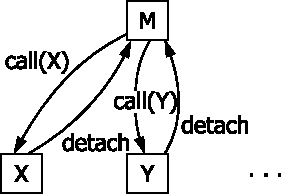
\includegraphics[width=\textwidth]{chap2/fig1}
	\caption{Representation of date (7, March, 1908)}
\end{figure}

A second occasion for using packed representations is when data storage is scarce, either in main store or on external backing stores. However, care must be taken that space saved on data storage is not outweighed by the expansion of the code which results from having to unpack and repack the data whenever it is inspected or updated.

The minimal representation is not often used for data storage, since the small amount of extra space it saves (always less than one bit per component) is usually more than outweighed by the extra time taken by multiplying and dividing on every access to the components, as compared with the more usual shifting and masking. However, the technique can be useful, possibly in conjunction with more conventional packing, if there is no other way of fitting the value within convenient word boundaries. Also, if the value is to be used solely or primarily as an index to a multi-dimensional array, the minimal representation is to be preferred; since this will save a significant amount of space in the representation of the array (see Section \ref{sec:representation-6.2}).

In representing the \textbf{with} construction in machine code, it is sometimes convenient to compute the address of the structure being referenced and store it in a register; this may achieve shorter and faster code for accessing the components. If the components have been packed, it may pay to unpack them into separate words before starting to process them, so that they can be easily referenced or updated; and if they have been updated, they must be packed up again and stored in the structure when the processing is complete. On some machines, it is more economic to pack and unpack a whole structure at the same time, rather than to perform these operations one at a time on the components.

\noindent
\textit{Exercise}
\nopagebreak

\noindent
Given a variable

\quad today:date;

\noindent
write a program to assign the value of the next following date to the variable tomorrow: date. Translate this program into the machine code of your choice using a tightly packed representation. Rewrite the program using an unpacked and then a minimal representation. Compare the lengths of the code involved, and the time taken to execute them.

\section[The discriminated union]{The Discriminated Union}

In defining sets of objects, it is often useful to define one set as the union of two previously known sets. For example, when jokers are added to a standard pack of cards, the extended set may be described as the union of the standard set plus the set consisting of the ``wild'' cards, joker I and joker 2. A type whose values range over the members of this set may be declared as the union of two alternatives, the card type, and an enumeration type with two distinct values:

\quad \textbf{type} pokercard $=$ (normal:($s$:suit; $r$:rank),

\tabto{10.2em}wild:(joker I, joker 2)).

\noindent
Each value of type pokercard corresponds either to an ordered pair with components indicating suit and rank; or else it corresponds to one of the two jokers in the enumeration type.

In specifying a constant of a discriminated union type, it is necessary to indicate to which of the alternative types the value denoted is intended to belong. This is done by writing the name of the alternative explicitly, for example:

\quad pokercard(normal(heart, Jack))

\noindent
denotes a value from the first alternative, whereas

\quad pokercard(wild(joker 2))

\noindent
denotes a value from the second alternative. In general, it is convenient to omit the type name, where the type can be inferred from context.

A second example of a discriminated union might be found in the maintenance of a register of all cars in a country. Cars may be distinguished as local cars owned by residents of the country, and visitor cars brought into the country temporarily by non-residents. The information required is rather different in the two cases. In both cases the number and the make of the car is considered relevant. However, for a local car, the name of the owner of the car is required, and the date on which the car was first registered in that owner's name. For visitor cars, this information is not relevant: all that is required is the standard three-letter abbreviation of the name of the country of origin. Thus the definition of the two alternative types of car might be:

\quad \textbf{type} local car = (make:manufacturer; regnumber:carnumber;

\tabto{9.4em} owner:person; first registration:date);

\quad \textbf{type} visitor car = (make:manufacturer; regnumber:carnumber;

\tabto{10.1em} origin:country);

Now it is possible to define a type covering both kinds of car:

\quad \textbf{type} car $=$ (local:local car,

\tabto{7.4em} foreign:visitor car).

\noindent
But here it is inconvenient to define the structure of local and foreign cars separately; and we would like to take advantage of the fact that several of their components are the same. This may be done by bringing the common components in front of both alternatives:

\quad \textbf{type} car $=$ (make:manufacturer;

\tabto{7.5em}regnumber:carnumber;

\tabto{7.5em}(local: (owner:person;

\tabto{7.8em}first registration:date),

\tabto{7.8em}foreign: (origin:country))

\tabto{7.1em}).

\noindent
Every car has a make and regnumber but only local cars have an owner or first registration date; and only foreign cars have an origin. 

A third example is the definition of geometric figures, which in some application might be categorized as either rectangles, triangles, or circles

\quad \textbf{type} figure $=$ (position:point; rect:$R$, tri:$T$, circ:$C$).

\noindent
The method of specifying the figure varies in each case. For a rectangle, the angle of inclination of one of the sides is given, together with the two lengths of the sides:

\quad \textbf{type} $R =$ (inclination:angle; side1, side2: real).

\noindent
A triangle is specified by the angle of inclination and length of one of its sides together with the angles formed between it and the other two sides:

\quad \textbf{type} $T =$ (inclination:angle; side:real; angle1, angle2:angle).

\noindent
For a circle, all that is necessary is to specify the diameter as a real number.

\quad \textbf{type} C $=$ (diameter:real).

When a type is defined as the union of several other types, it is important to recognize that its values must be considered wholly distinct from those of any of the types in terms of which it is defined. Otherwise there would be an immediate violation of the rule that each value belongs to only one type. Thus the union of types must be clearly distinguished from the normal concept of set union. Furthermore, for each element of the union type, it is possible to determine from which of the constituent types it originated, even if the same type has been repeated several times. For example, a double pack of cards used for playing patience may be defined as the union of two packs, i.e.,

\quad \textbf{type} patience card $=$ (red:cardface, blue:cardface).

\noindent
Each value of type patience card is clearly marked as having originated either from the red pack or from the blue pack, even if perhaps in the real world the colors of the backs are the same. This fact explains the use of the term ``discriminated union'' to apply to this form of type definition. It follows that the cardinality of a discriminated union is always the sum of the cardinalities of its constituent types.

\subsection{Manipulation}

Any value of a discriminated union carries with it a \textit{tag} field indicating which of the particular constituent types it originated from; on assignment this is copied, and on a test of equality, the tag fields must be the same if the values are to be equal.

On constructing a value of a discriminated union type, it is necessary to name the alternative type from which the value originated:
\smallskip

\quad patience card(red(spade, Jack)).
\smallskip

\noindent
This will automatically cause the value ``red'' to be assigned to the tag field of the result.

A particular car may be denoted by
\smallskip

\quad car(Ford, ``RUR157D'', local(me, date(1, Sept, 1968))).
\smallskip

In order to access and operate on the information encoded as a discriminated union, it is necessary to convert it back to its original type. This may be accomplished by the convention of using the label of this type as if it were a selector, e.g.:

card1.wild \tabto*{8em} is of type (joker 1, joker 2)

car1.foreign \tabto*{8em} is of type (origin:country)

fig1.tri \tabto*{8em} is of type $T$

\noindent
If the constituent type is a Cartesian product, its selectors may be validly applied to the resulting value, using the convention that the .operator associates to the left.

\quad card1.normal.$r$

\quad car1.local.owner

\quad fig1.circ.diameter

If the programmer attempts to convert a discriminated union value back to a type from which it did \textit{not} originate, this is a serious programming
error, which could lead to meaningless results. This error can be detected only by a runtime check, which tests the tag field whenever such a conversion is explicitly or implicitly invoked. Such a check is time consuming and when it fails, highly inconvenient. We therefore seek a notational technique which will guarantee that this error can never occur in a running program; and the guarantee is given by merely inspecting the text, without any knowledge of the runtime values being processed. Such a guarantee could be given by an automatic compiler, if available.

The proposed notational technique is a mixture between the \textbf{with} construction for Cartesian products and the case construction for discrimination. Suppose that a value $sv$ of union type is to be processed in one of several ways in accordance with which of the alternative types it came from. Then one may write

\quad \textbf{with} $sv$ \textbf{do} \{$a1:S_1$

\tabto*{7.6em}$a2:S_2$,
\smallskip

\tabto*{8.85em}\vdots

\tabto*{7.6em}$an:S_n$\};

\noindent
where $S_i$ is the statement to be selected for execution whenever the value of the tag field of $sv$ is $a_i$. Within $S_1$ it is guaranteed safe to assume that the value came from the corresponding alternative type, provided that the value of $sv$ remains unchanged. Consequently it is safe to use the component selectors which are defined for that alternative type by themselves to refer to the components of $sv$, just as in the case of a simple \textbf{with} statement described previously for a Cartesian product.

If it is desired to regard a union type as ordered, the most natural ordering is that defined by taking all values corresponding to earlier alternatives in the list before any of the values of the later alternatives.

\noindent
\textit{Exercise}
\nopagebreak

\noindent
Write a function that will compute the area of a figure as defined above.

\subsection{Representation}

In representing a value from a discriminated union it is necessary first to represent the tag as an integer between zero and $n - 1$, where $n$ is the number of alternative types. The tag is followed directly by the representation of the value of the original type. As with the Cartesian product, there is a choice of the degree of packing used in a representation.

In the unpacked representation the tag occupies a complete word, and the space occupied by each value of a union type is one word more than that occupied by values from the largest alternative type. In a packed representation, this overhead can be reduced to a few bits. In the minimal representation, each value is obtained by adding its minimal representation in the original type to the sum of the cardinalities of all preceding types in the union. Thus a value originating from the first type, for example (diamond, four), has exactly the same value as it has in the original type, namely 16. But joker 1, with value zero in the original enumeration type, has added to it the cardinality of the card type.

The choice between unpacked, packed and tight packed representations is based on the same considerations as for Cartesian products; however the runtime speed penalty for the minimal representation is a great deal less, since recovery of the original value requires only subtraction rather than division.

In general the values of the different alternative types occupy different amounts of storage, so the shorter values have to be ``padded out'' to equalize the lengths, thus observing the convenient rule that elementary data types occupy a fixed amount of storage. In later chapters it will be seen that this padding can often be omitted when the value is a component of some larger structure.

\begin{figure}[ht!]
	\centering
	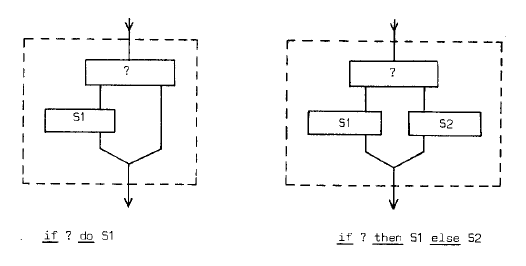
\includegraphics[width=.8\textwidth]{chap2/fig2}
	\caption{Representation of cars}
\end{figure}

In present-day programming practice, it is quite common to omit the tag field in the representation of unions. In order to operate correctly on such a representation, the programmer needs to ``know'' from other considerations what the interpretation of the value ought to be, since it is not possible to find out from the value itself. If his belief is mistaken, this is not detectable either by a runtime or compile-time check. Since the effect of such an error will depend on details of bitpattern representation, it will give rise to results unpredictable in terms of the abstractions with which the programmer is working. It would therefore in general seem advisable to use tag fields and compile-time checkable case discriminations as standard programming practice, to be bypassed only in exceptional circumstances.

\subsection{Example}

We return to the context of the example in section \ref{sec:example-3-3}, the analysis of language text into meaningful symbols. We wish to give a rigorous abstract definition of what these symbols are.

\quad \textbf{type} symbol $=$

\tabto*{5.7em}(realconst:real,

\tabto*{6em}integerconst:integer,

\tabto*{6em}identifier:ident,

\tabto*{6em}basic:delimiter);

\noindent
where we will leave the type ident undefined for the time being, and assume that the delimiters are defined by enumeration.

\section[The array]{The Array}
\label{sec:array}

The array is for many programmers the most familiar data structure, and in some programming languages it is the only structure explicitly available. From the abstract point of view, an array may be regarded as a mapping between a domain of one type (the subscript range) and a range of some possibly different type (the type of the array, or more accurately, the type of its elements).

The type of a mapping is normally specified by a mathematician using an arrow:

\quad $M:D\rightarrow R$;

\noindent
where $D$ is the domain type and $R$ is the range type. An alternative notation which will be more familiar to programmers is:

\quad M:\textbf{array} $D$ \textbf{of} $R$.

This notation is more expressive of the manner in which the data is represented, whereas the mathematical notation emphasizes the abstract character of the structure, independent of its representation.

When a particular value $M$ of a mapping type is applied to a value $x$ of the domain type, it specifies some unique element of the range type, which is known as $M$ of $x$, and is written using either round or square brackets

\quad $M(x)$ or $M[x]$.

\noindent
Another name for a mapping is a function: the term ``mapping'' is used to differentiate the data structure from a piece of program which actually computes a value in its range from an argument in its domain. The essence of the difference is that a mapping $M$ is specified not by giving a computation method but by explicitly listing the value of $M(x)$ for each possible value $x$ in its domain. Thus an array can be used only for functions defined at a finite set of points, whereas the domain of a computed function may be infinite.

An example of a finite mapping is a monthtable, which specifies for each month of the year the number of days it has:

\quad \textbf{type} monthtable $=$ \textbf{array} month \textbf{of} $28\,.\,.\,31$.

\noindent
The domain is the month type and the range type consists of the integers between 28 and 31 inclusive. A typical value of this type may be simply specified by listing the values of $M(x)$ as $x$ ranges over its domain. Thus if $M$:monthtable is specified as

\quad monthtable(Jan:31, Feb:28, March:31, April:30,

\quad May:31, June:30, July:31, Aug:31,

\quad Sept:30, Oct:31, Nov:30, Dec:31)

\noindent
then $M[\text{Jan}] = 31,\, M[\text{Feb}] = 28$, and so on.

The array provides a method of representing a particular arrangement of cards in a pack, since each arrangement may be regarded as a mapping which indicates for each of the fifty-two possible positions in a pack the value of the card which occupies that position. Thus each possible arrangement may be regarded as a value of the mapping type:

\quad \textbf{type} cardpack = \textbf{array} $1\,.\,.\,52$ \textbf{of} cardface.

\noindent
Of course, not all values of this type represent actual card packs, since there is nothing to prevent some value of the type from mapping two different positions onto the same card; which in real life is impossible.

Arrays with elements that are of Cartesian product type are sometimes known as \textit{tables}.

A third example of an array is that which represents all possible con- figurations of character punching on a conventional punched card. This may be regarded as a mapping $M$ which maps each column number into a character, namely the character punched in that column.

\quad \textbf{type} punchcard = array $1\,.\,.\,80$ \textbf{of} character.

\noindent
Any possible text punched into a card may be regarded as a single value of type punchcard.

A fourth example shows an array which represents a possible value of a page on a cathode ray tube display device. There are assumed to be 40 rows and 27 character positions in each row. The effect of two dimensions can be achieved by specifying the domain of the mapping as a Cartesian product of the possible rows and the possible character positions within each row. This is written as follows:

\quad \textbf{type} spot $=$ (row:$1\,.\,.\,40$; column:$1\,.\,.\,27$);

\quad \textbf{type} display page $=$ \textbf{array} spot of character.

An alternative method of dealing with a multidimensional array is to regard it as an array of rows, where each row is an array of characters:

\quad \textbf{type} display page $=$ \textbf{array} $1\,.\,.\,40$ \textbf{of} row;

\quad \textbf{type} row $=$ \textbf{array} $1\,.\,.\,27$ \textbf{of} character.

\noindent
This is a more suitable abstract structure if the rows are to be processed separately and the columns are not.

The cardinality of an array type is computed by raising the cardinality of the range type to the power of the cardinality of the domain type, i.e.

\quad cardinality$(D \rightarrow R) =$ cardinality$(R)^{\text{cardinality}(D)}$

\noindent
This may be proved by considering the number of decisions which have to be made to specify completely a value of an array type. For each value of the domain we have to choose between cardinality$(R)$ possible values of the range type. We have to make such a choice independently for each element of the array, that is cardinality$(D)$ times.

\subsection{Manipulation}

A mapping which maps all values of its domain onto the same value of its range is known as a constant mapping. A natural constructor for arrays is one which takes as argument an arbitrary range value, and yields as result the constant array, all of whose elements are equal to the given range value. It is convenient to use the type name itself to denote this constructor, e.g.

\quad $M = \text{monthtable}(31)$

\noindent
is an array such that $M[m] = 31$ for all months m.

\quad card pack(cardface(heart, King))

\noindent
is obviously a conjuror's pack.

The basic constructive operation on an array is that which defines a new value for one particular element of an array. If $x$ is a value of an array type $T$, $d$ a value from its domain type, and $r$ a value from its range type, then we write:

\quad $T(x, d:r)$

\noindent
to denote a value of type $T$ which is identical to $x$ in all respects, except that it maps the value $d$ into $r$. The $T$ may be omitted if its existence can be inferred from context. Similarly, the constant array $T(x)$ may be denoted by all $(x)$.

The basic selection operator on arrays is that of subscripting. This is effectively a binary operation on an array and a value from its domain type; and it yields the corresponding value of its range type.

The most common and efficient way of changing the value of an array is by selective updating of one of its components, which is accomplished by the usual notation of placing a subscripted array variable on the left of an assignment:

\quad $a[d]\coloneq r.$

\noindent
This means the same as

\quad $a\coloneq T(a, d:r).$

\noindent
Note that from an abstract point of view a new value is assigned to the whole array.

Normally an array type would be regarded as unordered; but in some cases, particularly character arrays, it is desirable to define an ordering corresponding to the normal lexicographic ordering; this is possible only when domain and range types are ordered. In this case the ordering of two arrays is determined by that of the lowest subscripted elements in which the two arrays differ. Thus

\quad ``BACK'' $<$ ``BANK''

\noindent
because the third letter is the first one in which they differ, and

\quad ``$C$'' $<$ ``$N$''

A convenient method of specifying an array value is by means of a \textit{for expression}, which is modeled on the for statement:

\quad \textbf{for} $i:D$ \textbf{take} $E$

\noindent
where $E$ is an expression yielding a value of the range type, and containing the variable $i$. As $i$ scans through the domain type $D$, evaluation of the expression $E$ yields the value of the corresponding element of the array.

If certain operations are defined on the range type of an array, it is natural to extend these operations to apply to the array type as well. For example, if $A$ and $B$ are real arrays with the same domain, it is natural to write

\quad $A + B,$ $A - B$,

to denote arrays (with the same domain) whose elements are the sum and difference of the values of the corresponding elements of $A$ and $B$. But the programmer must retain his awareness that these can be expensive operations if the arrays are large, and he should seek ways of eliminating the operations in progressing from an abstract to a more concrete program.

\subsection{Representation}
\label{sec:representation-6.2}

The representation of arrays in a computer store is familiar to most programmers. The most usual representation is the unpacked representation, which allocates one or more whole words to each element of the array. In this case, the computer address of each element is simply computed: first, the value of the subscript is converted to a minimal representation; then this is multiplied by the number of words occupied by each element; and finally the result is added to the address of the first element of the array. The normal word-selection mechanism of the computer can be used to access and update this value independently of the other elements of the array.

An alternative representation involves packing of elements within word boundaries, so that each element occupies only a certain fixed number of bits within a word, although the array as a whole may stretch over several words. In the example of a monthtable, each element can take only four values, 28 to 31; therefore it can be accommodated in only two bits in the minimal representation; the whole array can therefore be accommodated in twenty-four consecutive bits.

When an array is packed in this way, the task of selecting the value of a subscripted variable is far more complicated. In order to select the right word, the subscript (in minimal form) must be divided by the number of elements in each word. The quotient is added to the address of the first word of the array, which is then accessed. The remainder is multiplied by the number of bits in each element, and the result is used as a $\text{shift-count}_2$ to shift the required value into a standard position within the word. The unwanted values of neighboring elements of the array can then be masked off. The method of selectively updating an element of a packed array is even more laborious, since the new value must be inserted at the right position within the word, without disturbing the values of the neighboring elements. The efficiency of both operations may be slightly increased if the number of elements per word is an exact power of two, since then the integer division of the subscript may be replaced by a shift to find the quotient, and a mask to find the remainder. On some machines, further efficiency may be gained if each element is stored in a single character position.

The minimal representation for an array is similar to that for a Cartesian product, except that the multiplier of each element value is equal to the cardinality of range type, raised to the power of the subscript value. The process of selecting or updating a value of an element of an array stored in minimal representation is even more laborious than that described above, unless the cardinality of the range type is an exact power of two. It would be prohibitive if the array were to stretch over more than one normal computer word. For this reason, the minimal representation for arrays is of mainly academic interest.

\begin{figure}[h]
	\centering
	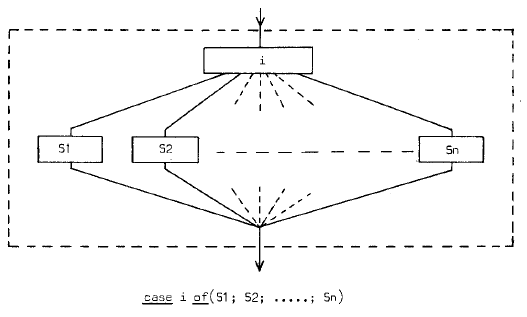
\includegraphics[width=\textwidth]{chap2/fig3}
	\caption{Representation of $A:\text{\textbf{array} } 0\,.\,.\,7 \text{ \textbf{of} } T$}
\end{figure}

When the domain of a finite mapping is itself a data structure, for example, a Cartesian product, it is usual to represent this domain in the minimal representation, so as to avoid allocation of unused storage space. For example, the display page has a domain which is the Cartesian product of the integer ranges 1 to 40 and 1 to 27. In the minimal representation, this gives a range of integers between 0 and $40 \times 27 - 1 = 1079$. Consequently 1080 consecutive words are allocated to hold values of elements of the array. In order to access any element in a given row and character position, it is necessary first to construct a minimal representation for the subscript, in the manner described in Section \ref{sec:representation-4-2}

An alternative method of representation of multidimensional arrays is sometimes known as a codeword or descriptor method, but we shall give it the title of ``tree representation''. The essence of the method is to allocate a single-dimensional \textit{base} array with one element corresponding to each row of the array, and to place in it the address of a block of consecutive storage locations which holds the values of that row. These rows do not have to be contiguous. Now the process of accessing or updating each element does not have to be done by computing a minimal representation of the subscript. All that is necessary is to add the row-number to the address of the first element of the base of the tree, and thus access the address of the first element of the required row, to which the value of the next subscript is added to give the address of the required element.

\begin{figure}[h]
	\centering
	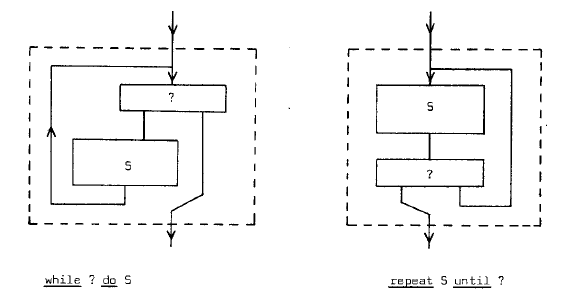
\includegraphics[width=\textwidth]{chap2/fig4}
	\caption{Representation of two-dimensional arrays}
\end{figure}

The choice between unpacked and packed representations of arrays is made on grounds similar to the choice in the case of a Cartesian product. The unpacked representation is used when fast access and updating is required; it is also the obviously appropriate choice when the range type naturally fits within computer word boundaries, for example if the elements are floating point numbers. The packed representation is recommended if the size of the elements is considerably shorter than a single word, and if storage is short, or if copying and comparison of the arrays is frequent compared with subscripting and selective updating. A particularly common case of packed arrays is the representation of identifiers in a programming language, where it is acceptable in the interests of efficiency to truncate identifiers which are too long to fit into the standard array, and pad out those that are too short with blanks.

The choice between representations of multidimensional arrays is made on quite different grounds. The standard representation is more economical of storage, and gives good efficiency on sequencing through elements of the array by rows, columns, or both. Furthermore, it is more convenient when the arrays must be transferred as a whole between main and backing store. However, on a machine with slow multiplication, it will be faster to use the tree representation, and accept the extra storage required to hold the array of addresses, which is small provided that the rows are not too short. If each row contains only two words, there would be a fifty per cent overhead on data storage.

There are several other possible reasons for choosing the tree representation:

\begin{enumerate}[leftmargin=2\parindent, label=(\arabic*)]
	\item In some computing environments, where dynamic storage allocation is standard, it may be difficult to obtain large consecutive areas, in which case a large two-dimensional array can be split up into a number of smaller rows which can be accommodated without trouble.

	\item It is possible to set up a scheme whereby some rows of the array are held on backing store while other rows are being processed, and then the backing store address of a row replaces the main store address in the base array when that row is absent from store. Thus it is hoped to be able to process arrays which are too large to be wholly accommodated in main store together with the program that processes them. However, the economics of this operation need to be carefully examined to ensure that the number of backing store transfers involved is acceptable.

	\item In some applications, it is known that several matrices share the same rows. In the tree representation it is possible to set up a single copy of such a shared row, and merely take copies of its address rather than its full value. But in such a case, the shared row must not be selectively updated.

	\item The tree representation is recommended even in the case of single-dimensional arrays if the size of the individual elements is highly variable; and on multidimensional arrays, if the length of the rows is highly variable.
\end{enumerate}

\noindent
\textit{Exercise}
\nopagebreak

\noindent
The character set of an input device includes only thirty characters, defined by enumeration; they include the characters space, newline, newpage. Characters may be read in one at a time from an input device to a buffer, using a procedure call

\quad read next character.

\noindent
They should be assembled line by line into an array

\quad page:display page,

\noindent
and on receipt of a newpage character, this should be output to a display device by the instruction

\quad outpage.

\noindent
The display device does \textit{not} recognize the characters newline or newpage; consequently the ends of lines and pages have to be filled up with spaces.

Write a program in a suitable language to perform this operation, using a selection of representations for the display page, e.g.

\quad unpacked

\quad loosely packed

\quad tightly packed

\quad indirect.

\noindent
Rewrite the program, using different representations. Compare the lengths and speeds of the code and data involved in the different representations.

Write the corresponding programs to read a page from the display, and output the individual characters, taking care to eliminate redundant spaces at the ends of each line and blank lines at the end of each page wherever possible.

\section[The powerset]{The Powerset}

The powerset of a given set is defined as the set of all subsets of that set; and a powerset type is a type whose values are sets of values selected from some other type known as the \textit{base} of the powerset. For example, the primary colors have been defined by enumeration as red, yellow and blue. The other main colors are made up as a mixture of two or three of these colors: orange is a mixture of red and yellow; brown is a mixture of all three primary colors. Thus each main color (including the primary colors) can be specified as that subset of the primary colors out of which it can be mixed. For example, orange may be regarded as the set with just two members, red and yellow. Using the traditional notation for sets defined by enumeration, this may be written: \{red, yellow\}. The pure color red may be regarded as the set whose only member is the primary color red, i.e. \{red\}. In this way it is possible to represent the seven main colors, red, orange, yellow, green, blue, purple and brown. When no primary color is present (i.e. the null or empty set) this may be regarded as denoting the absence of color, i.e. perhaps white. The type whose values range over the colors may be declared as the power set of the type primary color:

\quad \textbf{type} color $=$ \textbf{powerset} primary color.

A second example is provided by considering a data structure required to represent the status of the request buttons in a lift. A simple variable of type floor (see Section \ref{sec:unstructured-data-types}) is capable of indicating one particular stop of a lift.  But if we wish to record the status of the whole panel of buttons inside a lift, it would be necessary to represent this as a subset of all possible floors in the building, namely, the subset consisting of those floors for which a request button has been depressed. Thus the type liftcall may be defined as the powerset of the floor type:

\quad \textbf{type} liftcall $=$ \textbf{powerset} floor.

A third example is provided by a hand of cards in some card game, for example, poker or bridge. A hand is a subset of playing cards, without repetitions, and is therefore conveniently represented by a value from the powerset type:

\quad \textbf{type} hand $=$ \textbf{powerset} cardface;

\noindent
This type covers all hands of up to fifty-two cards, even though for a particular game there may be standard size of a hand, or a limit less than fifty-two.

A final example expresses the status of a computer peripheral device, for example, a paper tape reader. There are a number of exception conditions which can arise on attempted input of a character:

\begin{enumerate}[leftmargin=2\parindent, label=(\arabic*)]
	\item Device switched to ``manual'' by operator.
	\item No tape loaded.
	\item Parity error on last character read.
	\item Skew detected on last character read.
\end{enumerate}

\noindent
These conditions can be defined as an enumeration

\quad \textbf{type} exception $=$ (manual, unloaded, parity, skew); 

\noindent
and since several of these conditions can be detected simultaneously, the status of the reader can be specified as a value of a powerset type:

\quad \textbf{type} statusword $=$ \textbf{powerset} exception.

The cardinality of the powerset type is two raised to the power of the cardinality of the base type, i.e.

\quad cardinality $(\text{\textbf{powerset} } D) = 2^{\text{cardinality} (D)}$

This may be proved by considering the number of decisions which have to be made to specify completely a value of the type. For each value of the base type there are two alternatives, either it is in the set or it is not. This decision may be made independently cardinality $(D)$ times.

\subsection{Manipulation}

The basic construction operation on sets is the one that takes a number of values from the domain type, and converts them into a set containing just those values as members. As in the case of the Cartesian Product, the type name is used as the transfer function, but for sets, the number of arguments is variable from zero upwards. For example:

\quad primary color (red, yellow) \tabto*{14em} i.e. orange

\quad liftcall (ground) \tabto*{14em}  i.e. only a single button has been pressed

\quad statusword () \tabto*{14em} i.e. no exception condition.

\noindent
The last two examples illustrate the concept of a \textit{unit set} (which must be clearly distinguished from its only member) and the null or \textit{empty set}, which contains no member at all. If the type name is omitted in this construction, curly brackets should be used instead of round ones in the normal way.

The converse of the null set is the universal set, which contains all values from the base type. This may be denoted

\quad $T$.all.

\noindent
However, this universal set exists as a storable data value only when the base type is finite.

The basic operations on sets are very familiar to mathematicians and logicians.

\begin{enumerate}[leftmargin=2\parindent, label=(\arabic*)]
	\item Test of membership: If $x$ is in the set $s$, the Boolean expression ``$x$ \textbf{in} $s$'' yields the value true, otherwise the value false.
	\item Equality: two sets are equal if and only if they have the same members.
	\item Intersection: $s_1 \wedge s_2$ contains just those values which are in both $s_1$ and $s_2$.
	\item Unions: $s_1 \vee s_2$ contain just those values which are either in $s_1$ or $s_2$, or both.
	\item Relative complement: $s_1 - s_2$ contains just those members of $s_1$ which are not in $s_2$.
	\item Test of inclusion: $s_1 \subset s_2$ yields the value true whenever all members of $s_1$ are also members of $s_2$, and false otherwise.
	\item The size of a set tells how many members it has.
\end{enumerate}

If the domain type of a set has certain operators defined upon it, it is often useful to construct corresponding operations on sets. In particular, if the domain type of a set is ordered, the following operators apply:

\begin{enumerate}[leftmargin=2\parindent, label=(\arabic*)]
	\setcounter{enumi}{7}
	
	\item $\min(s)$ the smallest member of $s$; undefined if $s$ is empty.
	\item $s \text{ \textbf{down} } n$ is a set containing just those values whose nth successors are in $s$.
	\item $s \text{ \textbf{up} } n$ is a set containing just those values whose $n$th predecessors are in $s$.
	\item Range$(a, b)$ is the set containing a, succ$(a), \dots, b$ if $a \leqslant b$, and which is empty otherwise.
\end{enumerate}

The most useful selective updating operations on sets are:

\noindent
$x:\vee\ y$; \tabto*{5em} join the set $y$ to $x$

\noindent
$x:\vee\ T(a)$ \tabto*{5em} add the member $a$ to $x$

\noindent
$x:\wedge\ y$; \tabto*{5em} exclude from $x$ all members which are not also members of $y$

\noindent
$x:-\ y$ \tabto*{5em} exclude from $x$ all members which are also members of $y$

\noindent
\hangindent=3.2\parindent$x:\text{\textbf{down} }n$ \tabto*{5em} subtract n from every member of x and exclude members for which this is not possible

\noindent
\hangindent=3.2\parindent$x:\text{\textbf{up} } n$ \tabto*{5em} add $n$ to every member of $x$, and exclude members for which this is not possible

\noindent
It is also sometimes useful to select some member from $x$ and simultaneously remove it from $x$. This operation can be expressed by the notation:

\quad $a$ \textbf{from} $x$.

\noindent
If the domain type of $x$ is ordered, it is natural that the selected member should be the minimum member of $x$; otherwise the selection should be regarded as arbitrary.

It is often useful to define the value of a set by giving some condition $B$ which is satisfied by just those values of the domain type which are intended to be members of the set. This may be denoted:

\quad $\{i:D \mid B\}$

\noindent
where \tabto*{3em} $i$ is a variable of type $D$ regarded as local to $B$,

\noindent
and \tabto*{3em} $B$ is a Boolean expression usually containing and depending on $i$.

\noindent
In order for this expression to denote a value of the powerset type it is essential that the cardinality of $D$ be finite, and that $B$ is defined over all values of the type.

Finally, it is frequently required to perform some operation on each member of some set, that is to execute a loop with a counting variable which takes on successively all values in the set. A suitable notation for expressing this is:

\quad \textbf{for} $x$ \textbf{in} $s$ \textbf{do} \dots

\noindent
If the base type of $s$ is an ordered type, it seems reasonable to postulate that the elements will be taken in the natural order, starting with the lowest. For an unordered base type, the programmer does not care in which order the members are taken, and he leaves open the option to choose an order that contributes best to efficiency.

\subsection{Representation}

In choosing a computer representation for powersets, it is desirable to ensure that all the basic operations can be executed simply by single machine code instructions; and further, that the amount of store occupied is minimized. For most data structure storage methods, there is a fundamental conflict between these two objectives, and consequently a choice between representation methods must be made by the programmer; but in the case of powersets the two objectives can be fully reconciled, provided that the base type is not too large.

The recommended method of representation is to allocate as many bits in the store as there are potential members in the set. Thus to each value of the base type there is a single bit which takes the value one if it is in fact a member, or zero if it is not. For example, each value of type color can be represented in three bits; the most significant corresponding to the primary color red, and the least significant corresponding to blue. Thus the orange color is represented as 110 and red as 100. Each set of size $n$ is represented as a bit pattern with exactly $n$ ones in the appropriate positions. The null set is accordingly represented as an all-zero bit pattern.

Another example is afforded by the ``hand'' type, which requires fifty-two bits for its representation, one corresponding to each value of type cardface. In this case, it is advisable to use the minimal representation of the base type, to avoid unused gaps in the bit pattern representation.

Since the number of values of a powerset type is always an exact power of two, for powersets of small base there can be no more economical method of utilizing storage on a binary computer than that of the bit pattern representation. It remains to show that the operations defined over the powerset type can be executed with high efficiency.

\begin{enumerate}[leftmargin=2\parindent, label=(\arabic*)]
	\item The unitset of $x$ may be obtained by loading a single 1 into the signbit position, and shifting it right $x$ places. On computers on which shifting is slow, the same effect may be obtained by table lookup. The construction of a set out of components may be achieved by taking the logical union of all the corresponding unit sets.

	\item A membership test $x$ \textbf{in} $s$ may be made by shifting $s$ up $x$ places and looking at the most significant bit: 1 stands for \textbf{true} and 0 for \textbf{false}.

	\item Logical intersection, union, and complementation are often available as single instructions on binary computers.

	\item The size of a set can sometimes be discovered by a builtin machine code instruction for counting the bits in a word. Otherwise the size can be determined by repeated standardization, masking off the next-to-sign bit on each occasion. A third method is to split the bitpattern into small parts, and use table lookup on each part, adding together the results.

	\item The \textbf{up} and \textbf{down} operations can obviously be accomplished by right or left shifts.

	\item The min of a set can be efficiently discovered by a standardize instruction, which automatically counts the number of shifts required to move the first one-bit into the position next to the sign.

	\item The for statement may also be efficiently constructed using standardization, masking off each one-bit as it is reached.

	\item The range operation can be accomplished by two shifts, the first of which regenerates the sign bit.	
\end{enumerate}

Thus when the cardinality of the domain type is not greater than the number of bits. in the largest computer word to which logical and shift operations can be applied, all these operations can be carried out with great efficiency. If significantly more than one such word is involved, it will usually pay to use selective updating operations rather than the normal result-producing operators. Furthermore, operations such as size and min can become rather inefficient, and it will often pay to store these values redundantly together with the set, and keep them up to date whenever the value of the set is updated, rather than recomputing them whenever they are required.

When it is known that the cardinality of the base type is very large (perhaps even infinite) compared with the size of the typical set, the bitpattern representation altogether loses its attraction, since it no longer pays to store and operate upon large areas of zeroes. The treatment of such sparse sets is postponed to Section \ref{sec:sparse-data-structures}

\subsection{Example}

\noindent
\textit{Problem}: Write a program to construct a set

\quad primes:\textbf{powerset} $2\,.\,.\,N$;

\noindent
containing all prime numbers in its base type.

\noindent
Use the method of Eratosthenes' sieve to avoid all multiplications and divisions.

The method of Eratosthenes is first to put all numbers in the ``sieve'' and repeat the following until the sieve is empty:

\noindent
Select and remove the smallest number remaining in the sieve (necessarily a prime), and then step through the sieve, removing all multiples of that number.

The program can be written easily

\noindent
\textbf{begin} $n$, next:$2\,.\,.\,N$; sieve:\textbf{powerset} $2\,.\,.\,N$;

\noindent
\quad sieve $\coloneq$ range$(2, N)$;

\noindent
\quad primes $\coloneq$ \{\};

\noindent
\quad \textbf{while} sieve $\neq$ empty \textbf{do}

\noindent
\quad \quad \textbf{begin} next $\coloneq$ min(sieve);

\noindent
\quad \quad \quad primes:$\vee$ \{next\};

\noindent
\quad \quad \quad \textbf{for} $n\coloneq$ next \textbf{step} next \textbf{until} $N$ \textbf{do}

\noindent
\quad \quad \quad \quad sieve:$-\ \{n\}$

\noindent
\quad \quad \textbf{end}

\noindent
\textbf{end} primefinder.

But if $N$ is significantly large, say of the order of 10\,000, this program cannot be directly executed with any acceptable degree of efficiency. The solution is to use this program as an abstract model of the algorithm, and rewrite it in a more efficient fashion, using only operations on sets not exceeding the word-length of the computer. We therefore need to declare an array of words to represent the two sets, assuming that ``wordlength'' is an environment inquiry giving the number of bits in a word:

\quad primes, sieve:\textbf{array} $0\,.\,.\,W$ \textbf{of powerset} $0\,.\,.\,\text{wordlength} - 1$

\noindent
where $W = (N + 1) \div \text{wordlength} + 1$.

\noindent
This means that the two sets may be slightly larger than $N$, but for convenience we shall accept that harmless extension.

In order to access an individual bit of these sets, it is necessary to know both the wordnumber and the bitnumber. Since we do not wish to use division to find these, we will represent the counting variables $n$ and next as Cartesian products

\quad $n$, next:$(w,\ b$:integer$)$;

\noindent
where $w$ indicates the wordnumber and $b$ indicates the bitnumber.

It is now as well to check the efficiency of this representation by recoding the innermost loop first.

\quad \textbf{for} $n\coloneq$ next \textbf{step} next \textbf{until} $N$ \textbf{do} sieve:$-\ \{n\}$;

\noindent
is recoded as :

\quad $n\coloneq$ next;

\quad \textbf{while} $n.w \leqslant W$ \textbf{do}

\quad \quad \textbf{begin} sieve$[n.w]$:$-\ \{n.b\}$;

\quad \quad \quad $n.b\coloneq n.b + \text{next}.b$;

\quad \quad \quad $n.w\coloneq n.w + \text{next}.w;$

\quad \quad \quad \textbf{if} $n.b \geqslant$ wordlength \textbf{then begin} $n.w \coloneq n.w + 1$;

\quad \quad \quad \quad $n.b \coloneq n.b - \text{wordlength}$

\quad \quad \quad \textbf{end}

\quad \quad \textbf{end}

\noindent
Since this appears acceptably efficient we will code the other operations of the outer loop, starting with the most difficult:

\quad next $\coloneq$ min(sieve);

\noindent
Here we do not wish to start our search for the minimum at the beginning of the sieve set each time, since towards the end of the process this would involve scanning many empty words. We therefore take advantage of the fact that the new value of next must be larger than the old value.

The search consists of two parts, first finding a nonempty word, and then its first bit. But if the search for a word reaches the end of the array, the whole program is completed

\quad \textbf{while} sieve$[\text{next}.w] = \{\}$ \textbf{do} $\{\text{next}.w \coloneq \text{next}.w +1$;

\quad \quad \textbf{if} next.$w > W$ \textbf{then exit} primefinder$\}$;

\quad \quad next.$b\coloneq$ min$(\text{sieve}[\text{next}.w])$;

The remaining operations are trivial. Since the outer loop is terminated by an exit, there is no need to test a separate while condition; and the statement

\quad primes:$\vee$ \{next\};

\noindent
can be coded as

\quad primes$[\text{next}.w]$:$\vee\ \{\text{next}.b\}$.

The whole program including initialisation is as follows:

\quad primes, sieve: \textbf{array} $0\,.\,.\,W$ \textbf{of powerset} $0\,.\,.\,\text{wordlength} - 1$;

\quad \textbf{begin} primefinder;

\quad \quad $n$, next:$(w, b$:integer$)$;

\quad \quad \textbf{for} $t$:$0\,.\,.\,W$ \textbf{do begin} primes$[t] \coloneq \{\}$;

\quad \quad \quad sieve$[t] \coloneq$ range $(0\,.\,.\, \text{wordlength} - 1)$

\quad \quad \textbf{end};

\quad \quad sieve$[0]$:$-\ \{0, 1\}$;

\quad \quad next.$w\coloneq 0$;

\quad \quad \textbf{while} true \textbf{do}

\quad \quad \quad \textbf{begin while} sieve$[\text{next}.w] = \{\}$ \textbf{do}

\quad \quad \quad \quad \textbf{begin} next.$w\coloneq$ next.$w + 1$;

\quad \quad \quad \quad \quad \textbf{if} next.$w > W$ \textbf{then exit} primefinder

\quad \quad \quad \quad \textbf{end};

\quad \quad \quad \quad next.$b\leqslant$ min(sieve$[\text{next}.w])$;

\quad \quad \quad \quad primes$[\text{next}.w]$:$\vee\ \{\text{next}.b\}$;

\quad \quad \quad \quad $n\leqslant$ next;

\quad \quad \quad \quad \textbf{while} $n.w \leqslant W$ \textbf{do}

\quad \quad \quad \quad \quad \textbf{begin} sieve$[n.w]$:$-\ \{n.b\}$;

\quad \quad \quad \quad \quad \quad $n.b\coloneq n.b + \text{next}.b$;

\quad \quad \quad \quad \quad \quad $n.w\coloneq n. w + \text{next}.w$;

\quad \quad \quad \quad \quad \quad \textbf{if} $n.b \geqslant$ wordlength \textbf{then}

\quad \quad \quad \quad \quad \quad \textbf{begin} $n.w\coloneq n.w + 1$;

\quad \quad \quad \quad \quad \quad \quad $n.b\coloneq n.b - \text{wordlength}$

\quad \quad \quad \quad \quad \quad \textbf{end}

\quad \quad \quad \quad \quad \textbf{end}

\quad \quad \quad \textbf{end}

\quad \textbf{end} primefinder

One feature of this program is that it uses an environment inquiry word length to achieve the full efficiency of which a machine is capable, and yet does so in a completely machine-independent fashion. The program will not only work, but work with high efficiency, on machines with widely varying word lengths.

But the most interesting feature about the program is the way in which it is related to the previous version. From an abstract point of view it expresses an identical algorithm; all that has changed is the manner in which the data has been represented on the computer. The original design acted as a framework or pattern, on which the more intricate coding of the second version was structured. By carrying out the design in two stages, we simplify the task of ensuring that each part of the final program works successfully in conjunction with the other parts.

\noindent
\textit{Exercise}
\nopagebreak

\noindent
Rewrite the program using sets representing only the odd numbers. (Hint: rewrite tile more abstract program first.)

\section[The sequence]{The Sequence}

The previous chapters have dealt with the topic of elementary data structures, which are of great importance in practical programming,  and present very little problem for representation and manipulation on modern digital computers. Furthermore, they provide the essential basis on which all other more advanced structures are built.

The most important distinction between elementary structured types and types of advanced structure is that in the former case the cardinality of the type is strictly finite, provided that the cardinality of the constituent types is. The distinction between a finite and an infinite set is one of profound mathematical significance, and it has many consequences relating to methods of representation and manipulation.

\begin{enumerate}[leftmargin=2\parindent, label=(\arabic*)]
	\item Since the number of potential values of the type may be infinite, the amount of storage allocated to hold a value of an advanced structure is not determinable from the declaration itself. It is normally only determined when the program is actually running, and in many cases, varies during the execution of the program. In the case of an elementary structure, the number of different potential values is finite, and the maximum amount of storage required to hold any value is fixed and determinable from the form of the declaration.

	\item When the size of a structured value is fairly large, it is more efficient to update individual components of the structure separately, rather than to assign a fresh value to the entire structure. Even for elementary types, it has been found sometimes more efficient to perform selective updating, particularly for unpacked representations of Cartesian products and for arrays. The increased efficiency of selective updating is usually even more pronounced in the case of advanced data structures.

	\item Advanced data structures, whose size varies dynamically, require some scheme of dynamic storage allocation and relinquishment. The units of storage which are required are usually linked together by pointers, sometimes known as references or addresses; and their release is accomplished either by explicitly programmed operations, or by some form of general garbage collection. The use of dynamic storage allocation and pointers leads to a significant complexity of processing, and the problems can be particularly severe when the data has to be transferred between the main and backing store of a computer. No problems of this kind need arise in the case of elementary data structures.

	\item The choice of a suitable representation for an advanced data structure is often far more difficult than for an elementary structure; the efficiency of the various primitive operations depends critically on the choice of representation, and therefore a sensible choice of representation requires a knowledge of the relative frequency with which these operations will be invoked. This knowledge is especially important when a part or all of the structure is held on a backing store; and in this case, the choice of re presentation should take into account the characteristics of the hardware device; that is, arrangement of tracks and cylinders on a rotating medium, and times of head movement and rotational delay. In the case of elementary structures, the primitive operations are of roughly comparable efficiency for most representations.
\end{enumerate}

Thus the differences between advanced and elementary structures are quite pronounced, and the problems involved are significantly greater in the advanced case. This suggests that the practical programmer would be well advised to confine himself to the use of elementary structures wherever possible, and to resort to the use of advanced structures only when the nature of his application forces him to do so.

The first and most familiar example of an advanced data structure is the sequence. This is regarded as nothing but a sequence of an arbitrary number of items of some given type. The use of the term ``sequence'' is intended to cover sequences on magnetic tapes, disc, or drum, or in the main store. Sequences in the main store have sometimes been known as streams, lists, strings, stacks, deques, queues, or even sets. The term file (or sequential file) is often used for sequences held on backing store. The concept of a sequence is an abstraction, and all these structures may be regarded as its various representations.

Our first example of a sequence is the string, familiar to programmers in ALGOL and SNOBOL. Since a string is constructed as a sequence of characters of arbitrary length, it may be defined:

\quad \textbf{type} string $=$ \textbf{sequence} character.

The next example is drawn from a data processing application; the maintenance of a file of data on cars. Each item of the file (sometimes known as a record) represents a single car, and is therefore of type car; an example of a possible definition of the car type has been given previously:

\quad \textbf{type} car file $=$ \textbf{sequence} car.

The third example gives an alternative method of dealing with a pack of cards. This may be regarded as just a sequence of cards, of length which perhaps varies as the cards are dealt:

\quad \textbf{type} deck $=$ \textbf{sequence} cardface;

\noindent
Of course, not all card-sequences represent actual decks of cards in real life; for example, sequences which contain the same card twice are invalid, and should be avoided by the programmer. Thus the maximum length of a valid deck is 52, although this fact is not expressed in the declaration.

The next example is drawn from the processing of a particular class of symbolic expression, namely the polynomial. A polynomial

$a_n x^n + a_{n-1}x^{n-i}\dots a_1 x + a_0$

\noindent
can be represented as the sequence of its coefficients a1• If the degree n of the polynomial is unpredictable or variable during the course of a calculation, a sequence is the most appropriate method of defining it:

\quad \textbf{type} polynomial $=$ \textbf{sequence} integer.

Our final example shows how it is possible to represent the programming language concept of the identifier. Since in theory an identifier may be of arbitrary length, a sequence is required. The items of the sequence are either letters or digits. However, the first character is always alphabetic and may be separated from the rest. Thus an exact definition of a data structure corresponding to the identifier is:

\quad \textbf{type} identifier $= ($first:letter; rest:\textbf{sequence} $(l$:letter, $d$:digit$))$.

\subsection{Manipulation}

The zero element of a sequence type $T$ is the sequence that contains no items --- this is known as the null or empty sequence, and is denoted by $T()$. For each value $v$ of the domain type, there is a sequence whose only item is $v$; this is known as the \textit{unit sequence} of $v$ and is denoted by $T(v)$. Finally, if $v_1, v_2, \dots, v_n$ are values from the base type (possibly with repetition),
$T(v_1, v_2, \dots, v_n)$ denotes the sequence consisting of these values in the stated order. If for convenience the type name $T$ is omitted, we will use square brackets to surround the sequence:

\quad $[v],$\qquad $[v_1, v_2, \dots, v_n]$

\noindent
However, a sequence of characters is normally denoted by enclosing them in quotes.

The basic operation on sequences is concatenation, that is, adjoining two sequences one after the other. Thus if $x$ is the sequence of characters ``PARIS IN THE'' and $y$ is the sequence ``THE SPRING'', their concatenation $\wideparen{xy}$ is the sequence

\quad $z =$ ``PARIS IN THETHE SPRING''

\noindent
Unless the operands are exceptionally small, concatenation is very inefficient on a computer, since it usually involves making fresh copies of both operands. The programmer should therefore make every effort to replace concatenation by selective updating.

The basic operators for breaking down a sequence into its component parts are those that yield the first and last items of a non-empty sequence

\quad $x$.first, $x$.last

\noindent
and those that remove the last or first items of a non-empty sequence, yielding the initial or final segments.

\quad initial$(x)$, final$(x)$.

An important relationship between sequences is that one sequence $x$ is equal to some initial or final subsequence of a sequence $y$:

\quad $x$ \textbf{begins} $y$

\quad or $x$ \textbf{ends} $y$.

\noindent
In our previous example, ``PARIS'' \textbf{begins} $z$ and ``RING'' \textbf{ends} $z$. These two tests can be rather time-consuming in a running program, and should be avoided wherever possible.

A significant property of sequences is their length, i.e. the number of items they contain; this may be found for a sequence $x$ by the function length$(x)$.

For some purposes (e.g. the construction of a dictionary) it is useful to regard a sequence type as ordered in accordance with traditional lexicographic principles: as in the case of arrays, the order of two sequences is determined by the ordering of the first item in which they differ; or if there is no such item, a shorter sequence precedes the longer sequence which it begins, for example:

\quad ``ALPHA'' $<$ ``ALPHABET''.

\noindent
In this ordering every sequence has a successor, but only a small proportion have predecessors.

A most important selective updating operation on sequences is the appending of a new value $v$ to the end of an existing sequence $x$. This may be written:


\quad $x\wideparen{\text{: } T}(v)$;

\noindent
and corresponds to the familiar concept of writing a value v to a sequential file $x$. The operation corresponding to reading the beginning of a file $x$ is one which removes the first item of $x$ and assigns its value to some variable $v$. This may be written:

\quad $v$ \textbf{from} $x$;

\noindent
In some applications, it is useful to be able to read back the most recently written item from a sequence; this may be expressed

\quad $v$ \textbf{back from} $x$;

\noindent
and it removes the last item from $x$. This operation can be used to ``pop up'' the top item of a stack which has been ``pushed down'' by an ordinary writing operation:

\quad $x\wideparen{\text{: } T}(v).$

\noindent
If desired, it is possible to define the fourth updating operation, that of attaching a new value to the beginning of a sequence. (putback($x$, $v$)).

In some cases, it is more efficient to avoid the copying of an item which is involved in the \textbf{from} operation. These cases may be dealt with by merely omitting the left hand variable, e.g.

\quad \textbf{from} $x$

\quad \textbf{back from} $x$.

\noindent
In this case, access to the items of the sequence will usually be made by the selectors $x$. first and$/$or $x$. last.

It is very common to wish to scan all the items of a sequence in succession; a suitable notation for this is modeled on the for statement:

\quad \textbf{for} $v$ \textbf{in} $x$ \textbf{do} $S$;

\noindent
If $x$ is empty, the statement is omitted. Otherwise the variable $v$ (regarded as local to $S$) takes in succession the values of all items from the sequence $x$, and $S$ is executed once for each value. In this construction neither $x$ nor $v$ should be updated within $S$.

A similar construction can be used for defining a sequence as an item-by-item transformation $E(v)$ of items $v$ in sequences.

\quad \textbf{for} $v$ \textbf{in} $s$ \textbf{take} $E(v)$.

In deciding a representation for a sequence, it is most important to know which of the selective updating operations are going to be carried out upon it.

\begin{enumerate}[leftmargin=2\parindent, label=(\arabic*)]
	\item If the only operation is \textbf{from}, the sequence is known as an \textit{input} sequence; obviously in order to have any value at all, an input sequence must be initialized to some value existing in the outer environment in which it is declared. The association of a sequence local to a program with some file existing more or less permanently on backing store is often known as ``opening'' the file for input, and we assume that this operation is invoked implicitly on declaration of a local input sequence. The reverse operation of ``closing'' the file is invoked implicitly on exit from the block to which the sequence is local.

	\item If the only operation is writing to the file, the sequence is known as an \textit{output} sequence. An output sequence may be initialized from the environment in the same way as an input sequence; or more commonly, it may take an empty initial value. In either case, in order to serve any useful purpose, the final value of the sequence on exit from the block must be assigned to some variable existing in the outer environment in which the sequence is declared. The identity of this outer variable should be declared together with the sequence; if this outer variable is held more or less permanently on backing store, it is known as an output file; and the rules for implicit invocation of opening and closing of the file on entry and exit to the block are similar to those for input files.

	\item If the only operations are writing and reading back (push down and 	pop up), the sequence is known as a \textit{stack}; the initial value of a stack is always empty, and the final value is not usually preserved. 

	\item If the only operations are writing to the end and reading from the beginning, the sequence is known as a \textit{queue}; again, the initial value is always empty, and the final value is not usually preserved.

	\item If reading and writing at both ends of a sequence are permitted, the sequence is sometimes known as a \textit{deque} (double-ended queue). However, to make all four operations equally efficient requires some complexity of representation, so it is fortunate that most programs can get by without using deques.
\end{enumerate}

\subsection{Representation}

\subsubsection{Contiguous representation}

The simplest method of representing a sequence is to allocate to it a fixed contiguous area of storage, adequate to hold all items actually required. This method is suitable if the value (or at least the length) of the sequence is constant throughout the execution of the program --- for example, a string of characters intended to be used as an output message or title.

In some cases, the length of the sequence is unknown at the time the program is written, but is known on entry to the block in which the sequence is declared, and this length remains constant throughout the existence of the sequence. In such cases, it is possible to allocate a contiguous area of storage in the local workspace of the block, using the standard stack method of store allocation and deallocation.

Even if the length of the sequence is subject to variation, it is sometimes possible to place an acceptably small upper bound on its length, and allocate permanently this maximum area. If the limit is exceeded during a run of the program, the programmer must be willing to accept its immediate termination. In addition to the fixed area, a pointer or count is required to indicate the current beginning and end of the sequence. In the case of a stack, the first item is always at the beginning, and only one pointer to the top of the stack is required. In the case of a queue, the sequence will at times overlap the end of the store area, and be continued again at the beginning. Such a representation is known as a cyclic buffer, and may be used in a parallel programming situation to communicate information between processes running in parallel. In this case, when a writing process finds the buffer full, it has to wait until a reading process reduces the size of the sequence again. Similarly, the reading process must wait when the buffer is empty.

Another case where the contiguous representation is the best is when the program requires only a single sequence, which may therefore occupy the whole of the remaining store available after allocation to other purposes; and if overflow occurs, the program could not have been run anyway. If two stacks are required, they can both be accommodated by arranging that one of them starts at one end of remaining available store and grows upwards, and the other starts at the other end and grows downwards. If the stacks meet, the program cannot continue.

If many sequences are to be represented, it is possible to set up a scheme in which they are spread through the remaining available store; and if any of them grows to meet its neighbor, it is possible to reshuffle some or all of the sequences, so that they all have sufficient room to grow again for a bit. For each sequence there must be a \textit{base location} pointing to its beginning, through which that sequence is always addressed. In addition, the actual length of the sequence must be stored. The base location and length of the neighboring sequence must always be inspected when the sequence is extended. When reshuffling takes place, the base locations of all moved sequences are updated to point to the new position of the sequence. This is quite a useful ad hoc scheme in cases where the reshuffling is known to be relatively infrequent; otherwise non-contiguous representations are to be preferred.

\begin{figure}[h]
	\centering
	\includegraphics[width=\textwidth]{chap2/fig5}
	\caption{Sequences (Contiguous representation)}
\end{figure}

When the individual items of a sequence are of variable length, there is usually no need to pad the shorter items out to the maximum length, since the use of the tag field, or other technique, will indicate the length of any given item, and this can be used to step the pointer by the right amount when the item is read. But this requires that the direction of reading be known at the time of writing, as in a stack or a queue. If reading is to be carried out from both ends, it will be necessary to ensure that the length of an item can be deduced from its bottom as well as its top, which will involve storing redundant information (e.g. length of previous item) between each item in the sequence.

\begin{figure}[h]
	\centering
	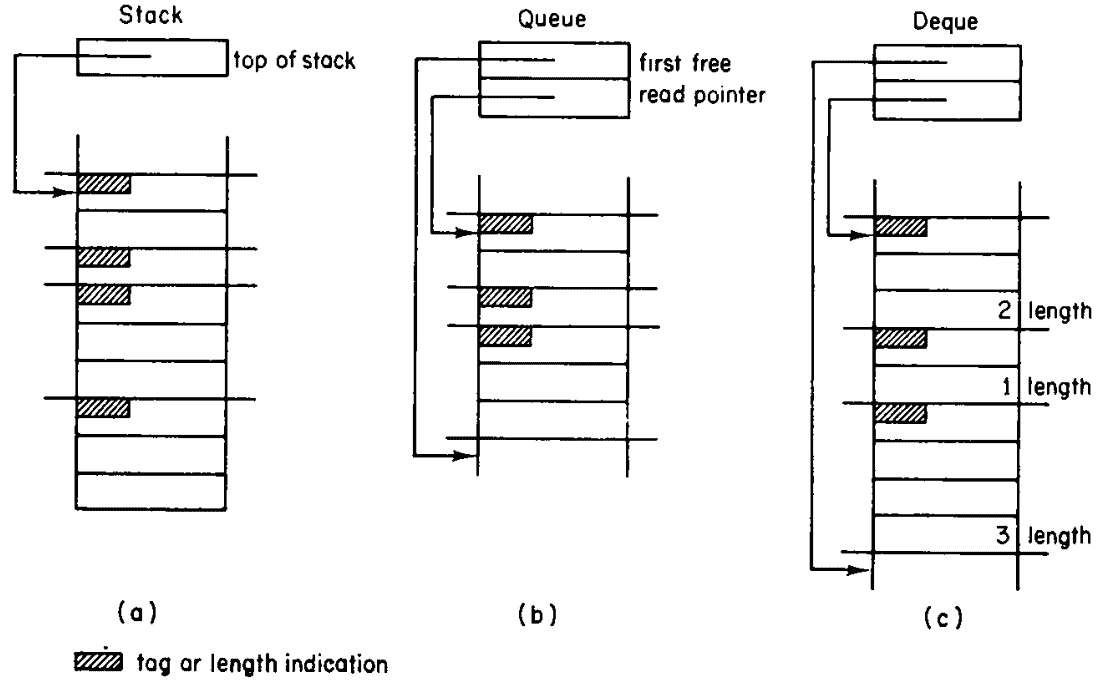
\includegraphics[width=\textwidth]{chap2/fig6}
	\caption{Sequences (variable length items)}
\end{figure}

When a sequence is itself a part of an item of some other sequence, the contiguous representation of the item-sequence may be used. This will normally be accompanied by a count giving the length of the sequence, so that the actual size of each item can be computed when the item is read.

\subsubsection{Chained representation}

In order to avoid reshuffling problems mentioned in the previous section, it is usual to introduce indirect or chained methods of storage allocation, using either fixed length or variable length units of allocation. The available store is split into areas, some of which will be in use for storing items of some sequence, and others will be free. The free areas are also linked together as a chained sequence. Whenever a programmer's sequence requires extension, an area (or part of an area) is acquired from the free chain; and whenever a sequence is shortened by reading, an area can be returned to the free chain. In the case of fixed-length items, the administration of dynamic storage allocation with explicit deallocation presents no problems. The problems of variable length allocation will not be treated here; they are best avoided by the use of blocking (see next section).

The simplest form of chain is the single linked chain. Each item of the sequence has adjoined to it, in a link location, the address of the next item in the chain. The empty sequence is represented by a value which could not possibly be an address (say zero or minus one); and the link location of the last item in the sequence contains this value. The first item in the chain is pointed to by the base location of the sequence.

A single linked chain is useful when the direction in which the sequence will be read is known; for the links have to point in this direction. In the case of a stack they will point backwards, and in the case of input and output sequences and queues they will point forwards. In the case of an input or output sequence, the base location of the external variable which is to hold the initial and$/$or final value of the sequence points permanently at the beginning of the chain, while the base location of the sequence itself steps through the sequence. In the case of a queue, two base locations are used, to point to each end of the sequence.

\begin{figure}[h]
	\centering
	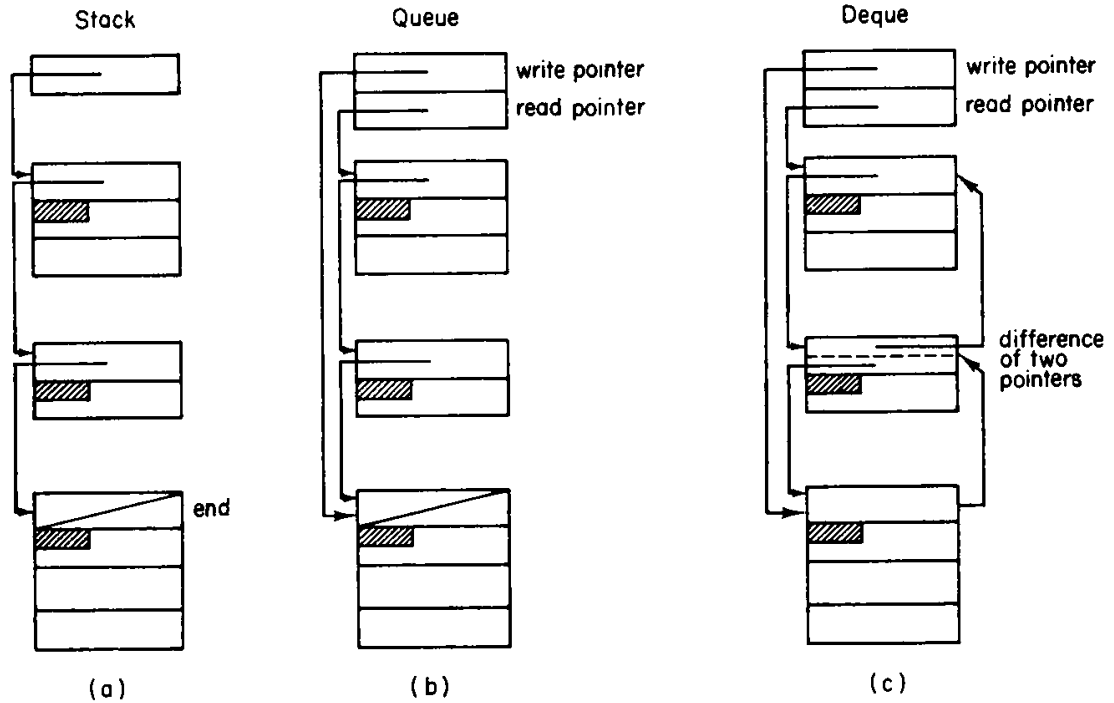
\includegraphics[width=\textwidth]{chap2/fig7}
	\caption{Sequences (Chained representation)}
\end{figure}

One possible advantage of the single-chained representation in the case of stacks is that several stacks can share the same initial segments, which may save space and time in some applications. However, when an item is popped up from such a stack, the storage space which it occupies cannot be immediately returned to the free chain, since it may be in use as part of another stack. One solution to this problem is never to return storage explicitly, but to wait until the free chain is exhausted. Then all currently allocated sequences are scanned, and all blocks currently in use are marked. Then all unmarked blocks are collected onto the free chain. This is known as a scan-mark-collect garbage collection. Although it appears to relieve the programmer of the responsibility of explicit control of main store allocation and deallocation, this can be dangerous in non-trivial computer applications where the responsibility is one that cannot so lightly be evaded.

In the case of a deque, when reading is required in both directions, a single-linked chain is no longer adequate; and the usual solution is to adjoin \textit{two} pointers to each item in the chain, one pointing to the previous item and one pointing to the following item. In fact these two pointers can be compressed into a single word containing only the difference between them. Since in the first and last items one of the pointers is a standard null value, the value of the other pointer from these items can always be obtained by subtraction. On reading or writing, the value of the link location for the new first or last item can be readily adjusted, since at this stage the address of the previous first or last item is still known. The detailed working out of this scheme is left as an exercise.

An alternative method of linking the items of a chain is to collect all links together in a single contiguous table, preferably of fixed length. This gives a form of tree representation for the sequence, and permits ready scanning in both directions. But it places an upper bound on the number of items in the sequence; and it means that the locations used for links must be permanently allocated, even at times when the sequence is relatively short. This problem can be mitigated by the use of blocking.

\subsubsection{Blocked representation}

One disadvantage of chaining is the amount of extra storage required to hold the links, and the time taken to administer the free store chain on each operation. These problems are particularly severe when the size of the individual items of the sequence are small and the sequence is long. The method of solving this problem is to use blocking; that is, a combination of the contiguous and chained techniques.

In this technique, a fixed-length block of storage is allocated, sufficient to hold perhaps between ten and a hundred items. When this block is filled, a new block is chained to it, using any of the methods described in the previous section. On input, a block is not released to free store until all the items it contains have been scanned. Thus the amount of store used on links can be reduced to negligible proportions. This can be of particular benefit in the tree representation of the chain.

As mentioned above, the use of blocking can also avoid the problems arising from variable-length dynamic storage allocation, since the size of the block may be held constant for all sequences, independent of the size of their items. Furthermore, in cases where part or all of the sequence is to be held on backing store, the use of blocking is almost universally indicated, since backing store transfers can be very inefficient if the unit of transfer is too small. The only (dubious) disadvantage of blocking is that it inhibits effective sharing of the tails of stacks.

The only remaining problem is to choose a size of block suitable for all purposes. It must obviously be large enough to accommodate the largest item of any sequence. In fact, it should be large enough to accommodate at least ten typical items; otherwise the space left over at the end of a block which is not large enough to accommodate the next item may reach significant proportions. Also, if the sequence is to be held partially or wholly on backing store, the block should be long enough to ensure that not too much space is wasted on interblock gaps, and the frequency of transfers is low enough to ensure that not too much time is spent in start-stop, latency, or head movement delays.

On the other hand, if the block size is too large, the space wasted at the beginning of the first block $\text{and}/\text{or}$ the end of the last block will become significant; thus the block size should be small enough to ensure that the typical sequence occupies at least ten blocks.

In the presence of so many conflicting considerations, it is not easy to select a standard block size for sequences of differing length and item size, and all forms of backing store, with different methods of access. However, an acceptable compromise can often be made, and on present-day computer designs, a block size of between 128 and 1024 words will often be a suitable choice. Probably in most cases the size chosen is not critical within a factor of two either way.

\subsubsection{Backing store representation}

In processing a sequence, a program normally requires access to one of its ends, and all the material in the middle and other end is unused for relatively long periods of time. If main storage is at all scarce, it is very profitable to transfer this material to backing store, so that the space it occupies in main store may be used for other purposes. In the case of input and output sequences, which have a lifetime greater than the program which reads or writes them, the use of backing store for long-term storage is almost obligatory.

When using backing store, efficiency of processing and representation demands that transfers should occur in blocks of reasonable size. The block which contains an active end of a sequence is always held in main store; and to permit overlap of input$/$output with computing, the previous block (on writing) or the next block (on reading) also remains allocated during the transfer operation. This is known as double-buffering. It is possible to hold even more buffers in store to smooth out variations in the speed of processing and the speed of transfer; but the program designer must not fall into the trap of supposing that this will help when there is a basic mismatch in the speeds of processing and transfer. In general, if double or triple buffering is inadequate, it is not worth while filling the store with any further extra buffers.

In a machine which is endowed with an automatic paging scheme, the problems of representing sequences are very much reduced. As far as the programmer is concerned, he need only allocate the amount of storage required for the longest possible sequence, using the contiguous representation. This should not actually cause any waste of storage, since the paging system should delay allocation of store until it is first used. As the sequence expands, new blocks of store will be allocated, but the addressing of these blocks will appear contiguous to the programmer, so there is no problem of leaving unused space at the end of blocks which are not large enough to hold the next item. Shortly after a block has been filled, it will automatically migrate to backing store; and it will be brought back again automatically as soon as it is required. On input sequences, a block which has been scanned will also be removed shortly afterwards from main store; but this will not involve an unnecessary backing store transfer if the material has not been changed since the last input took place. The only operation which a paging system will not perform automatically is to read a block of an input sequence into store ahead of its actual requirement.

\section[Recursive data structures]{Recursive Data Structures}

There are certain close analogies between the methods used for structuring data and the methods for structuring a program which processes that data. Thus, a Cartesian product corresponds to a compound statement, which assigns values to its components. Similarly, a discriminated union corresponds to a conditional or case construction, selecting an appropriate processing method for each alternative. Arrays and powersets correspond to for statements sequencing through their elements, with an essentially bounded number of iterations.

The sequence structure is the first that permits construction of types of infinite cardinality, with values of unbounded length; and it corresponds to the unbounded form of looping, with a \textbf{while} condition to control termination. The reason why the sequence is unbounded is that one of its components (i.e. the initial segment) from which it is built up belongs to the same type as itself, in the same way as the statement which remains to be obeyed after any iteration of a \textbf{while} loop is the same statement as before.

The question naturally arises whether the analogy can be extended to a data structure corresponding to recursive procedures. A value of such a type would be permitted to contain more than one component that belongs to the same data type as itself; in the same way that a recursive procedure can call itself recursively from more than one place in its own body. As in the case of recursive procedures such a structure can conveniently be defined by writing the name of the type being defined actually inside its own definition; or in the case of mutually recursive definition, in the definition of some preceding type.

The most obvious examples of recursive data structures are to be found in the description of arithmetic or logical expressions, programming languages, where the recursion reflects the possibility of nesting one expression inside another. For example, an arithmetic expression might be defined as follows:

``An expression is a series of terms, each of which consists of a sign $(+ \text{ or } -)$ followed by a sequence of factors. Each factor except the first consists of a sign $(x \text{ or } /)$ followed by a primary. A primary is either a constant, a variable, or an expression surrounded by brackets. An initial plus sign in an expression may be omitted.''

A structured data type whose values comprise such expressions may be defined using only techniques already familiar, plus recursion:

\quad \textbf{type} expression $=$ \textbf{sequence} term;

\quad \textbf{type} term $=$ (addop:operator; $f$:\textbf{sequence} factor);

\quad \textbf{type} factor $=$ (mulop:operator; $p$:primary);

\quad \textbf{type} primary $=$ (const:(val:real),

\tabto*{9.3em}var:($id$:identifier),

\tabto*{9.3em}bracketed:($e$:expression));

\quad type operator = (plus, minus, times, div);

This definition expresses the abstract structure of an arithmetic expression, but not the details of its concrete representation as a string of characters. For example, it does not specify the symbols used for brackets or operators, nor does it state whether an infix, prefix or postfix notation is used for them. It does not state how the three kinds of primary are to be distinguished. It does not even represent the optional omission of plus on the first term of an expression, and the necessary omission of $x$ on the first factor of a term. Apart from this degree of abstraction and representation-independence, this type definition would correspond to a set of BNF syntax equations:
\begin{bnf*}
	\bnfprod{expression}
	{\bnfpn{term} \bnfor \bnfpn{addop}\bnfpn{term} \bnfor \bnfpn{expression}\bnfpn{addop}\bnfpn{term}}\\
	\bnfprod{term}
	{\bnfpn{primary} \bnfor \bnfpn{term}\bnfpn{mulop}\bnfpn{primary}\\
	\bnfprod{primary}
	{\bnfpn{unsigned real number} \bnfor \bnfpn{variable} \bnfor (\bnfpn{expression})}}
\end{bnf*}

Note how we have used sequences to replace the recursion wherever possible. In fact this can be done whenever a type name occurs recursively only once at the beginning or at the end of its definition. For example:

\quad \textbf{type} expression $=$ \textbf{sequence} term;

\noindent
might have been formulated recursively:

\quad \textbf{type} expression $=$ (empty:(), non-empty:(first:term; final:expression)).

\noindent
A similar alternative formulation permits \textbf{while} loops to be expressed as recursive procedures.

The construction of values of a recursively defined type requires no new operators or transfer functions; all that is needed is recursive use of the methods defined for the other relevant structuring methods. For example, the expression
$$
3/(b - 2)
$$

\noindent
could be specified by the cumbersome construction:

\quad [term {plus, [factor (times, primary (const(3))),

\quad \quad factor (div, primary (bracketed (

\quad \quad \quad [term (plus, [factor (times, primary (var(``$b$'')))]),

\quad \quad \quad\hspace{.1em} term (minus, [factor (times, primary (const(2)))])])))

\quad \quad ])

\quad ].

\noindent
An effective method of getting the computer itself to translate expressions into abstract structures will be given as an example in (\ref{sec:example-9-2})

Another familiar example of recursively defined data is the family tree. A family tree (excluding information about marriage) can be defined by associating with each person the family trees of all his$/$her offspring. We assume that certain additional personal details are required to be held: 

\quad \textbf{type} family $=$ (head:person; offspring:\textbf{sequence} family);

A person with no children is an ultimate component of the family tree, and may be represented:

\quad family(Tom, [])

\noindent
A family with three children may be represented:

\noindent
family (Jill, [family (Tom, []),

\tabto{3.2em} family (Joanna, []),

\tabto{3.2em} family (Matthew, [])]).

The final example shows how the binary forking tree familiar to LISP programmers may be defined as a recursive data structure.

\quad \textbf{type} list = (atom:\textbf{sequence} character, cons:(car, cdr:list)).

\noindent
A list which in LISP dot-notation would be expressed

\quad ((A.(B.NIL)).NIL)

\noindent
can be expressed as a value of type list in almost exactly the same way as it is in LISP:

\quad cons (cons (atom (``A''),

\tabto{5em} cons (atom (``B''), atom (``NIL''))),

\tabto{5em} atom (``NIL'')

\tabto{4.8em} );

\noindent
where the type transfer to list type is left implicit.

As an example of the processing of a list, we write a function to reverse a complete tree, so that every ``left fork'' in it becomes a ``right fork'' and vice-versa.

\quad \textbf{function} reverse$(l$:list$)$: list;

\quad \quad \textbf{with} $l$ \textbf{do}

\quad \quad \quad \{atom:reverse$\coloneq l$,

\quad \quad \quad cons: reverse $\coloneq$ cons(reverse(cdr), reverse (car))\}

\subsection{Representation}

The standard representation of a recursive type is also very similar to that of a similarly structured non-recursive type, with the exception that each component specified as belonging to the recursive type itself is represented by a location containing a pointer to its value, rather than the value itself. This use of a pointer is motivated by the fact that the component value may be of arbitrary size; and it is not possible to allocate any fixed amount of storage to contain it. This is known as the ``tree representation'', and is similar to the tree representation of an array or sequence, except that the branches may grow to arbitrary and varying heights.

An alternative method of representation is the linear sequence or \textit{bitstream}. In this representation it is possible to avoid the use of pointers, and place the values of recursive substructures contiguous with the rest of the information, just as they are in the familiar bracketed character representations of expressions. However instead of using brackets, we can reestablish the bracketing structure by context, and if necessary by scanning the tag of union values. This method is usually associated with packed representations of the other components, and a very significant reduction in storage may be achieved, at the expense of enforcing serial access to the components of the structure. In many circumstances, a bitstream representation is some ten times more compact than the tree representation.

\begin{figure}[h]
	\centering
	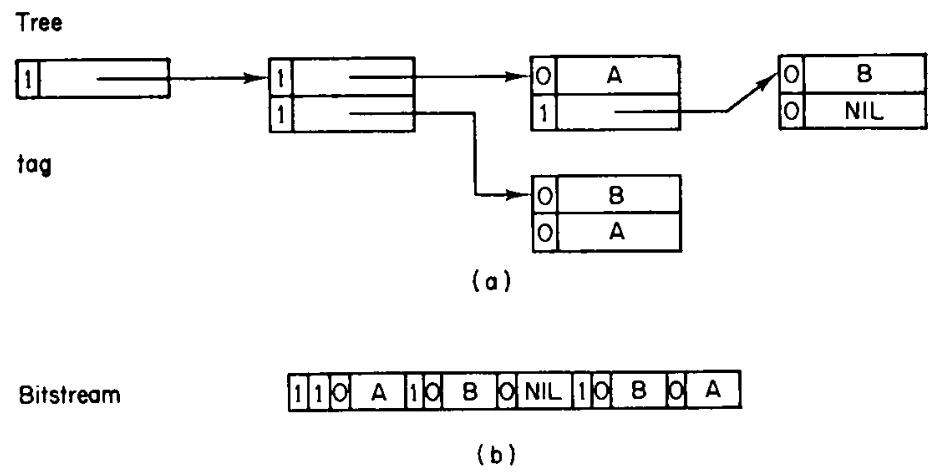
\includegraphics[width=.8\textwidth]{chap2/fig8}
	\caption{Representation of (($A$\,.\,($B$.NIL))\,.\,($B$\,.\,$A$)}
\end{figure}

The choice between tree and linear representation is usually obvious. If the structure is being processed by the program, usually by means of recursive procedures, the needs of ready access to any component of the structure dictate a tree representation. In addition, some of the space lost may be regained by sharing common branches among several trees; such commonality of branches is a feature of the processing of symbolic expressions. However, if the structure has to be output and subsequently re-input, the linear structure is vastly preferable. Not only does the reduction in volume reduce transfer time, but the linearization avoids a number of tricky problems of representing pointers in backing store. In many cases, a structure which passes through several phase~ of processing and input-output will be translated between the two representations at each phase; and this is standard practice in a multi-pass translator for a high-level programming language.

It is important to note that the sharing of the recursive sub-structure is nothing but a means of saving time and storage, and has no effect on the running of the program. This means that the sharing must be avoided whenever there is any danger that the shared sub-structure might be selectively updated as part of one of its owners. In principle, all values are entirely disjoint from all other values, and there is no way in which the programmer could either know or care how far his structures are shared. Furthermore, there is no way whatsoever in which a pointer can be made to point back to a structure of which it is a component; since this would mean that the structure was identical to one of its own components. Only an infinite structure can have this property; and infinite structures do not satisfy the axiom of exclusion on which the important principle of induction for recursive structures is based.

\subsection{Example}
\label{sec:example-9-2}

A source text for an expression in a programming language is presented as a sequence of symbols defined:

\quad \textbf{type} symbol $=$ (constant:(value:real), variable:(identifier: ident),

\tabto*{9.2em}op:operator, leftbracket, rightbracket);

Write a program operating on an input variable

\quad source:\textbf{sequence} symbol,

\noindent
which reads from its beginning the longest possible legitimate expression, delivers the corresponding abstract expression as a result, and exits to the label error if this is impossible. The structure of the result and the syntax of the source are as specified earlier in this chapter.

The structure of the program closely follows that of the desired result. There are three functions:

\quad compile expression

\quad compile term (sign)

\quad compile primary

\noindent
each of which removes from the source the longest expression in its syntactic category, and delivers the corresponding abstract structure as a result. The main irregularity of the process is that the first term of an expression may be unsigned; this is why the sign is provided as a parameter for compile term, instead of being read from source by compile term itself. Each function has the side-effect of shortening the source sequence if successful, and jumping to error if not.

\noindent
\textbf{function} compile expression:expression;

\noindent
\quad \textbf{begin} sign:operator;

\noindent
\quad \quad \textbf{if} source.first $=$ plus $\vee$ source.first $=$ minus \textbf{then} sign \textbf{from} source

\noindent
\quad \quad \textbf{else} sign $\coloneq$ plus;

\noindent
\quad \quad \quad compile expression $\leqslant$ [compile term(sign)];

\noindent
\quad \quad \quad \textbf{while} source.first $=$ plus $\vee$ source.first $=$ minus \textbf{do}

\noindent
\quad \quad \quad \quad \textbf{begin} sign \textbf{from} source;

\noindent
\quad \quad \quad \quad \quad compile expression$\wideparen{\text{: [}}$compile term(sign)]

\noindent
\quad \quad \quad \quad \textbf{end}

\noindent
\quad \textbf{end};

\noindent
\textbf{function} compile term($s$:operator):term;

\noindent
\quad \textbf{begin} $p$:primary; sign:operator; $fs$:\textbf{sequence} factor;

\noindent
\quad \quad $p\coloneq$ compile primary;

\noindent
\quad \quad $fs \coloneq$ [factor(times, $p$)];

\noindent
\quad \quad \textbf{while} source.first $=$ times $\vee$ source.first $=$ div \textbf{do}

\noindent
\quad \quad \quad \textbf{begin} sign from source:

\noindent
\quad \quad \quad \quad $p\coloneq$ compile primary;

\noindent
\quad \quad \quad \quad $fs\wideparen{\text{: [}}$factor(sign, $p$)]

\noindent
\quad \quad \quad \textbf{end};

\noindent
\quad \quad compile term $\coloneq$ term($s$, $fs$)

\noindent
\textbf{function} compile primary: primary;

\noindent
\quad \textbf{begin} $s$:symbol;

\noindent
\quad \quad $s$ \textbf{from} source;

\noindent
\quad \quad \textbf{with} $s$ \textbf{do} \{constant:compile primary $\coloneq$ const(value),

\noindent
\quad \quad \quad variable:compile primary $\coloneq$ var(identifier),

\noindent
\quad \quad \quad leftbracket:

\noindent
\quad \quad \quad \textbf{begin from} source;

\noindent
\quad \quad \quad \quad compile primary $\coloneq$ bracketed(compile expression);

\noindent
\quad \quad \quad \quad $s$ \textbf{from} source;

\noindent
\quad \quad \quad \quad \textbf{if} $s \neq$ rightbracket \textbf{then go to} error

\noindent
\quad \quad \quad \textbf{end},

\noindent
\quad \quad \textbf{else go to} error\}

\noindent
\quad \textbf{end};

\noindent
\textit{Exercise}
\nopagebreak

\noindent
Write programs to convert an expression from tree representation to bitstream and back again.

\section[Sparse data structures]{Sparse Data Structures}
\label{sec:sparse-data-structures}

In dealing with representations of arrays and powersets, we have hitherto assumed that the base type of a powerset and the domain type of an array is reasonably small, so that it is possible to allocate a bit or larger area of store to hold the value of every potential element of the structure. The examples also were confined to such cases. In this chapter we investigate the consequences and problems which arise when the base or domain types are very large or infinite, and when the standard representations are therefore impossible.

The representation and manipulation of powersets and mappings with infinite domains can be accomplished, provided that consideration is restricted to sets with only a finite number of members, and mappings in which only a finite number of elements take significant values; where ``significant'' is defined as different from some specified null or default value. The powerset of an infinite set is obviously also infinite; but since each value of the powerset type contains only a finite number of elements, each value can be specified simply by listing those elements in a finite period of time, and the list will occupy only a finite amount of storage. Similarly, each value of a mapping type with infinite domain can be finitely specified by listing all elements of the domain which map onto significant values of the range type, together with the value mapped in each case. A type which is restricted in this way is known as \textit{sparse}.

In fact the concept of sparsity is not confined to infinite bases and domains; it may also be applied to very large but finite powersets, when the programmer knows that each actual set in which he is interested will contain only a very small proportion of the potential members. For example, the base type may contain hundreds of millions of values, but the programmer may know that he only has to deal with sets of less than a hundred in size, and perhaps most of them less than ten. It would be impossible to use the bitpattern representation, since this requires hundreds of millions of bits; but since each value actually used in a program contains only a few members, these members can readily be listed in a comparatively small amount of store. A powerset type of this sort is known as \textit{sparse}. Similarly, arrays with a very large domain, nearly all of which map onto the same default value of the range, are said to belong to a \textit{sparse array} type.

Sparse sets and arrays are frequently encountered in advanced data processing applications, and their representation and manipulation present a number of familiar problems. Our first example is the definition of a type whose values are sets of car numbers. The cardinality of the carnumber type is perhaps something like four thousand million; but the programmer wishes only to deal with sets of cars owned by a single person; most of these will have only one member, and very few will have more than ten. The carset type may therefore be declared as sparse powerset:

\quad \textbf{type} carset $=$ \textbf{sparse} powerset carnumber;

As an example of a sparse array, we may take the type of mappings between car owners and the set of cars they own. Each owner is represented by name and address; since these are of arbitrary length, the owner type may be defined:

\quad \textbf{type} owner $=$ \textbf{sequence} character;

\noindent
and has infinite cardinality. The required type is therefore declared as sparse:

\quad \textbf{type} carfile $=$ \textbf{sparse array} owner \textbf{of} carset.

In a data processing application, a variable of carfile type would be known as a \textit{random access} file, and the owner would be known as the \textit{key} element of the file.

The next two examples are drawn from numerical applications. A vector is a mapping from integers onto floating point numbers. A sparse vector is one in which most of the elements are zero; consequently its initial value will be the zero constant function, and all elements will remain zero unless an explicit assignment is made of a different value:

\quad \textbf{type} sparsevector $=$ \textbf{sparse array} integer \textbf{of} real.

\noindent
A sparse complex matrix may be defined in a similar way:

\quad \textbf{type} irregular matrix $=$ \textbf{sparse array} (row, column:integer) \textbf{of} complex.

The next example is taken from the field of the translation of programming languages to machine code. During the process of translation, the translator needs to know certain information about each identifier declared in the program, such as machine address allocated to the variable, its length and type, etc. This information is assumed to belong to a type decode. The type of an array which associates a decode with each identifier is given the name dictionary and is declared:

\quad \textbf{type} dictionary $=$ \textbf{sparse array} ident \textbf{of} decode

\noindent
Of course, the translator is interested in the decode only of those identifiers actually declared in the source program. For the vast majority of possible identifiers, the value given by any dictionary of this type will be that value of the decode type which indicates that the identifier was undeclared.

The final example is of a type that causes familiar problems in a commercial filing system and in real life --- that of multidimensional cross-classification. The customers of a firm are split up into a number of geographical areas; they are also classified in a number of classes, in accordance with the kind of product they purchase. On occasions it is required to access all customers in an area, sequencing through all classes; on other occasions to access all customers in a class, sequencing through the areas; and finally, it is sometimes required to process all customers of a given class in a given area. The abstract structure required to deal with this situation is a two-dimensional sparse array of sparse sets:

\quad \textbf{sparse array} ($c$:class; $a$:area) \textbf{of sparse powerset} customer.

A similar example may arise in the description of family relationship among persons:

\quad \textbf{type} children $=$ \textbf{sparse array} (mother, father:person) \textbf{of} 

\tabto*{9.2em}\textbf{sparse powerset} person:

\noindent
This array caters for multiple marriages better than the more tree-like representations of a family, which can be defined as a recursive structure.

In the case of sparse arrays, it is sometimes useful to regard them as partial rather than total mappings. A partial mapping is one which does not necessarily give a value for each member of its domain type. In other words, the actual domain over which it is defined is a subset of the domain type. For such an array type it is necessary to introduce an additional constant omega, denoting a mapping which is everywhere undefined. It is also useful to introduce a function

\quad domain$(x)$

\noindent
which delivers as result the set of subscripts for elements of $x$ which are actually defined. Thus the programmer can sequence through all the defined elements, or test whether a particular element is defined or not. Many of the examples quoted above might well have been declared as partial instead of sparse. In the case of a partial mapping, the default value does not have to be recorded.

\subsection{Representation}

\noindent
Sparse sets and arrays are usually represented by simply keeping a record of the default value and those members or elements which are significant; thus the representation borrows techniques which are used in the case of the sequence type to deal with structures of changeable size. A sparse set may be regarded as a special case of a sparse mapping, which maps all its members onto the Boolean value true, and all its non-members onto the default value false. Thus their representations are closely similar to those of sparse arrays, and do not require separate treatment.

A sparse mapping consists of a number of elements. Each element of the mapping is represented as the Cartesian product of its subscript and its value; in this case the subscript is known as the \textit{key}, and the value is known as the \textit{information} associated with the element, and the juxtaposition of the two will be known as an \textit{entry}. In the case of a set which is sparse, there is no need to record any information, since the presence of the key itself is sufficient to indicate that this value is a member of the set. Thus an entry for a sparse set consists only of a key.

\subsubsection{Sequential representation}

The simplest representation of a sparse array type is as a sequence of entries;
i.e.
sparse array D of R
is represented as if it had been declared
(default:R; s:sequence (key:D; information:R)).
One of the possible sequence representations must now be chosen, in
accordance with the same criteria that are used in the case of a sequence.
But when a sequence is used to represent a sparse array, the order of the
entries is immaterial, and does not have to reflect the relative times at which
the entries were made. Thus the entries are often sorted into order of their
key-value, particularly if this is the order in which they are going to be
scanned.
The chief disadvantage of the sequential representation is the length of
time taken to access the element corresponding to a random subscript. In
the case of structures of any great size, the program designer usually goes to
considerable trouble to ensure that entries are accessed in the same standard
order that they are stored in the sequence; and that if new entries are to be
inserted, these are also sorted and then merged with the original sequence.
Thus the standard commercial practice of batch processing and updating of
sequential files may be regarded as a practical implementation of the abstract
concept of a sparse array on the rather unsympathetic medium of magnetic
tape.

\subsubsection{Tabular Representation}

If there is an acceptably low upper limit $N$ to the number of entries in a sparse mapping, a great increase in speed of lookup can be achieved by the tabular representation, in which the sparse mapping

sparse array D of R

\noindent
is represented as a nonsparse array:

(default:R; occupied: powerset 0 . . N;

array 0 .. N of (key: D; information: R) ).

If all the significant entries are collected before they are used, the table can be sorted, and then the entry with a given key can be rapidly located by logarithmic search.

If access to the elements of the array is interleaved with addition of new entries, some form of hash-table technique is indicated. For this an arbitrary ``hashing'' function is chosen, which maps the domain type D into an integer in the range $0\,.\,.\,N$. When the entry is inserted, it is placed at this position in the table; so whenever that entry is accessed, use of the same hashing function will find it there. If that position is already occupied by an entry with a different key, some other vacant position in the table must be found. It is quite usual to search for such a vacant position in the next following locations of the table; but when the table is nearly full, this may cause undesirable bunching around an area of the table which happens to be popular. A solution to this problem is to choose $N + 1$ as a prime number, and to use a second hashing function to compute an arbitrary step length from any given key. The next position to try when any given position is full is obtained by adding the step length (modulo $N + 1$) to the previous position.

\subsubsection{Indexed representation}

The tabular method of storage is suitable only when the whole table can be
accommodated in the main store of the computer. In the common case
when this is not possible, a mixture of the tabular and sequential methods is
often used. In this a sparse array is represented as a table, each of whose
entries is a sequence:

\quad (default:$R$; table:\textbf{array} $1\,.\,.\,N$ \textbf{of}

\tabto*{10em}(max:$D$; seq:\textbf{sequence} (key:$D$; information:$R$))).

\noindent
Every entry is placed on that sequence $i$ such that its key fails between table $[i - 1]$.max (or $D$.min if $i = 1$) and table $[i]$.max. The table is sorted so that the appropriate sequence can be quickly located. This technique may be likened to the organization of a multi-volume encyclopedia, in which the keys of the first and last entries of each volume are indicated on the spine, so that the right volume can he quickly identified, without extracting the volumes from the shelf.

When using this representation, it is desirable to ensure that all sequences are of roughly the same length. Indeed, if disc backing store is used, it is very advantageous to ensure that each of them is fitted onto a single cylinder, so that a random access will not involve more than a single head movement. Thus, when one sequence gets too long, it must exchange material with the adjacent sequence. This involves extracting the entries with the largest and/or smallest keys, and is best done when all the sequences are sorted into order of key-value. The sorting and reshuffling is often carried out as a separate operation at regular intervals; and the general method of file organization is known as ``indexed sequential''.

Naturally in this method of representation, it is an advantage to keep the sequences as short as possible, say less than a single track on disk. Consequently, the table itself may get so large that it will no longer fit in main store. In this case the table itself is split up into sections, and a second-level table may be set up to point to its sections, using the same principle again. Thus at least two accesses to backing store will in general be required for each access to an element of the array, and it is strongly recommended to ensure that the sizes and location of the sequences and sections be chosen to correspond closely with the access characteristics of the storage medium.

\subsubsection{Locally dense representation}

A special case of a sparse array encountered in numerical computer applications is the sparse matrix. Quite frequently a sparse matrix can be split into submatrices, only a few of which contain significant non-zero entries. In this case, the matrix may be said to be locally dense, and should be represented and processed in a manner which takes advantage of this fact.

One method of achieving this is to store with each significant submatrix its position and size, and to represent the whole matrix as a table or sequence of such submatrices, where each submatrix is stored contiguously in the usual way, using multiplicative address calculation. However, the submatrices will in general be of different sizes, and if the size varies during the processing of the matrix, the problems will be quite severe. A possible way of dealing with sparse matrices is to split them into submatrices of standard size, say sixteen by sixteen, and set up a table of pointers to each of these submatrices. A submatrix that is wholly zero is represented by a null pointer and occupies no additional storage; otherwise, the submatrix is stored in the usual way, using the following method of address calculation.

Each access to the array involves first ``interleaving'' the bit values of the two subscripts, so that the least significant part of the result contains the least significant part of both subscripts. The more significant part of the result is then used to consult the table of addresses, to locate the desired submatrix, and the less significant part to find the position of the required element within the submatrix. This technique of interleaving subscripts may on some machines be more efficient than general multiplication. If some of the submatrices have to be held on backing store, this method of address calculation is particularly recommended, since it is equally efficient at processing the matrix by rows as by columns; and the method can then be recommended for all large arrays, whether sparse or not, particularly on a paged computer. The inventor of this method is Professor E. W. Dijkstra.

\subsubsection{Grid representation}

The phenomenon of cross-classification of files causes as many problems in a computer as it does in real life. It is usually solved by standardizing on one of the classifications which is most convenient, and accepting the extra cost of processing in accordance with the other classification, even if this involves resorting the file. Thus the sparse mapping

\quad \textbf{sparse array} ($i$:$D_1$; $j$:$D_2$) \textbf{of} $R$

\noindent
is represented as:

\quad \textbf{sparse array} $D_1$ \textbf{of} (\textbf{sparse array} $D_2$ \textbf{of} $R$)

However, it is also possible to deal with the two dimensions in a more symmetric fashion, using a method based on the chained representation of sequences. In this representation, each actually used value of $D_1$ is placed in one chain, and each actually used value of $D_2$ is placed in another. These are called \textit{border chains}. Each element of either border chain contains a base location pointing to a chained sequence of all elements with key values which fall into the class. Now each actual entry of the array has \textit{two} addresses attached; one points to the next item of the sequence which has the same classification according to $D_1$, and the other to the next item which has the same classification according to $D_2$. Thus each item may be pictured as residing on an intersection of the lines of a two-dimensional grid, with pointers leading across and downwards to the next item on the same row or the same column.

\begin{figure}[h]
	\centering
	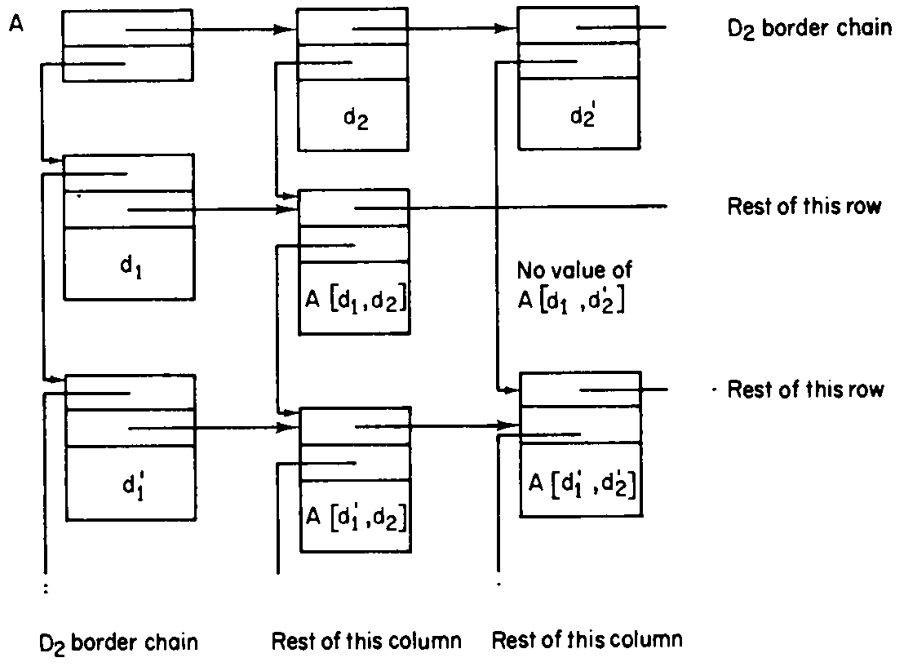
\includegraphics[width=.7\textwidth]{chap2/fig9}
	\caption{Grid representation of $A$: \textbf{sparse array} $(d_1: D_1;\ d_2: D_2)$ \textbf{of} $T$}
\end{figure}

This grid representation is unfortunately suitable only when the entire structure will fit into main store. If the main part of the sequences have to be held on backing store, some sort of blocking of adjacent elements would be desirable in the interests of efficiency.

\section[Example: Examination timetables]{Example: Examination Timetables}

In an educational establishment which offers students a wide choice of course combinations, there arises the problem of designing an examination timetable in which each examination is conducted in a single session, and yet each student can attend the examination for each course that he has taken. This can always be arranged by allocating a separate session for each examination; but the interests of examiner and student alike dictate that the total examination period be as short as possible. This means that each session should contain as many examinations as possible, subject to some limit $k$. An additional constraint is imposed by the size of the examination hall, which can only accommodate a certain maximum number of students.

Before designing the program, it is desirable to confirm our understanding of the problem by making a more rigorous formalization in terms of the structure of the various items of data, both given and required. The types ``student'' and ``exam'' are obviously unstructured and need no further definition at this stage. The load of exams to be taken by each student is given by a mapping:

\quad load:\textbf{array} student \textbf{of powerset} exam.

\noindent
A timetable is a set of sessions, where each session consists of a set of exams:

\quad \textbf{type} session $=$ \textbf{powerset} exam;

\quad timetable:\textbf{powerset} session.

\noindent
We next attempt to formalize the properties which the input and output data are required to possess.

\begin{enumerate}[leftmargin=2\parindent, label=(\arabic*)]
	\item We choose not to formalize the condition that the number of sessions be minimized, since in fact we do not want an absolute minimum if this turns out to be too expensive to compute.

	\item \label{en:examination-2}
	Each exam is scheduled for one of the sessions

	$\displaystyle\bigcup_{s\text{ \textbf{in} timetable} } $\quad $s =$ exam.all
	s in timetable

	\item \label{en:examination-3}
	No exam is scheduled for more than one session:

	\quad $(s1 \wedge s2 = \{\})$ or $(s1 = s2)$
\end{enumerate}

\noindent
Conditions \ref{en:examination-2} and \ref{en:examination-3} effectively state that the timetable is a partitioning of the set of all exams into exhaustive and exclusive subsets.

\begin{enumerate}[leftmargin=2\parindent, label=(\arabic*)]
	\setcounter{enumi}{3}
	
	\item No session includes more thank exams

	\quad $s$ \textbf{in} timetable $\supset$ size$(s) \leqslant k$

	\item No session involves more than hall size students. To formalize this, we need to count the number of students taking each exam:
	
	\quad examcount$(e:\text{exam}) = $size $\{st$:student $\mid$ $e$ \textbf{in} load$(st)\}$.
	
	Now the number of students involved in a session is
	
	\quad session count$(s\text{:session}) = \displaystyle\sum_{e \text{ \textbf{in} } s}$ examcount($e$)
\end{enumerate}

Page 157